\section{The Features}
\subsection{The Feature Distribution}\label{subsec:Dist}
\begin{figure}[H]
    \makebox[0.95\linewidth][c]{%
    \centering
    \begin{subfigure}{.405\textwidth}
        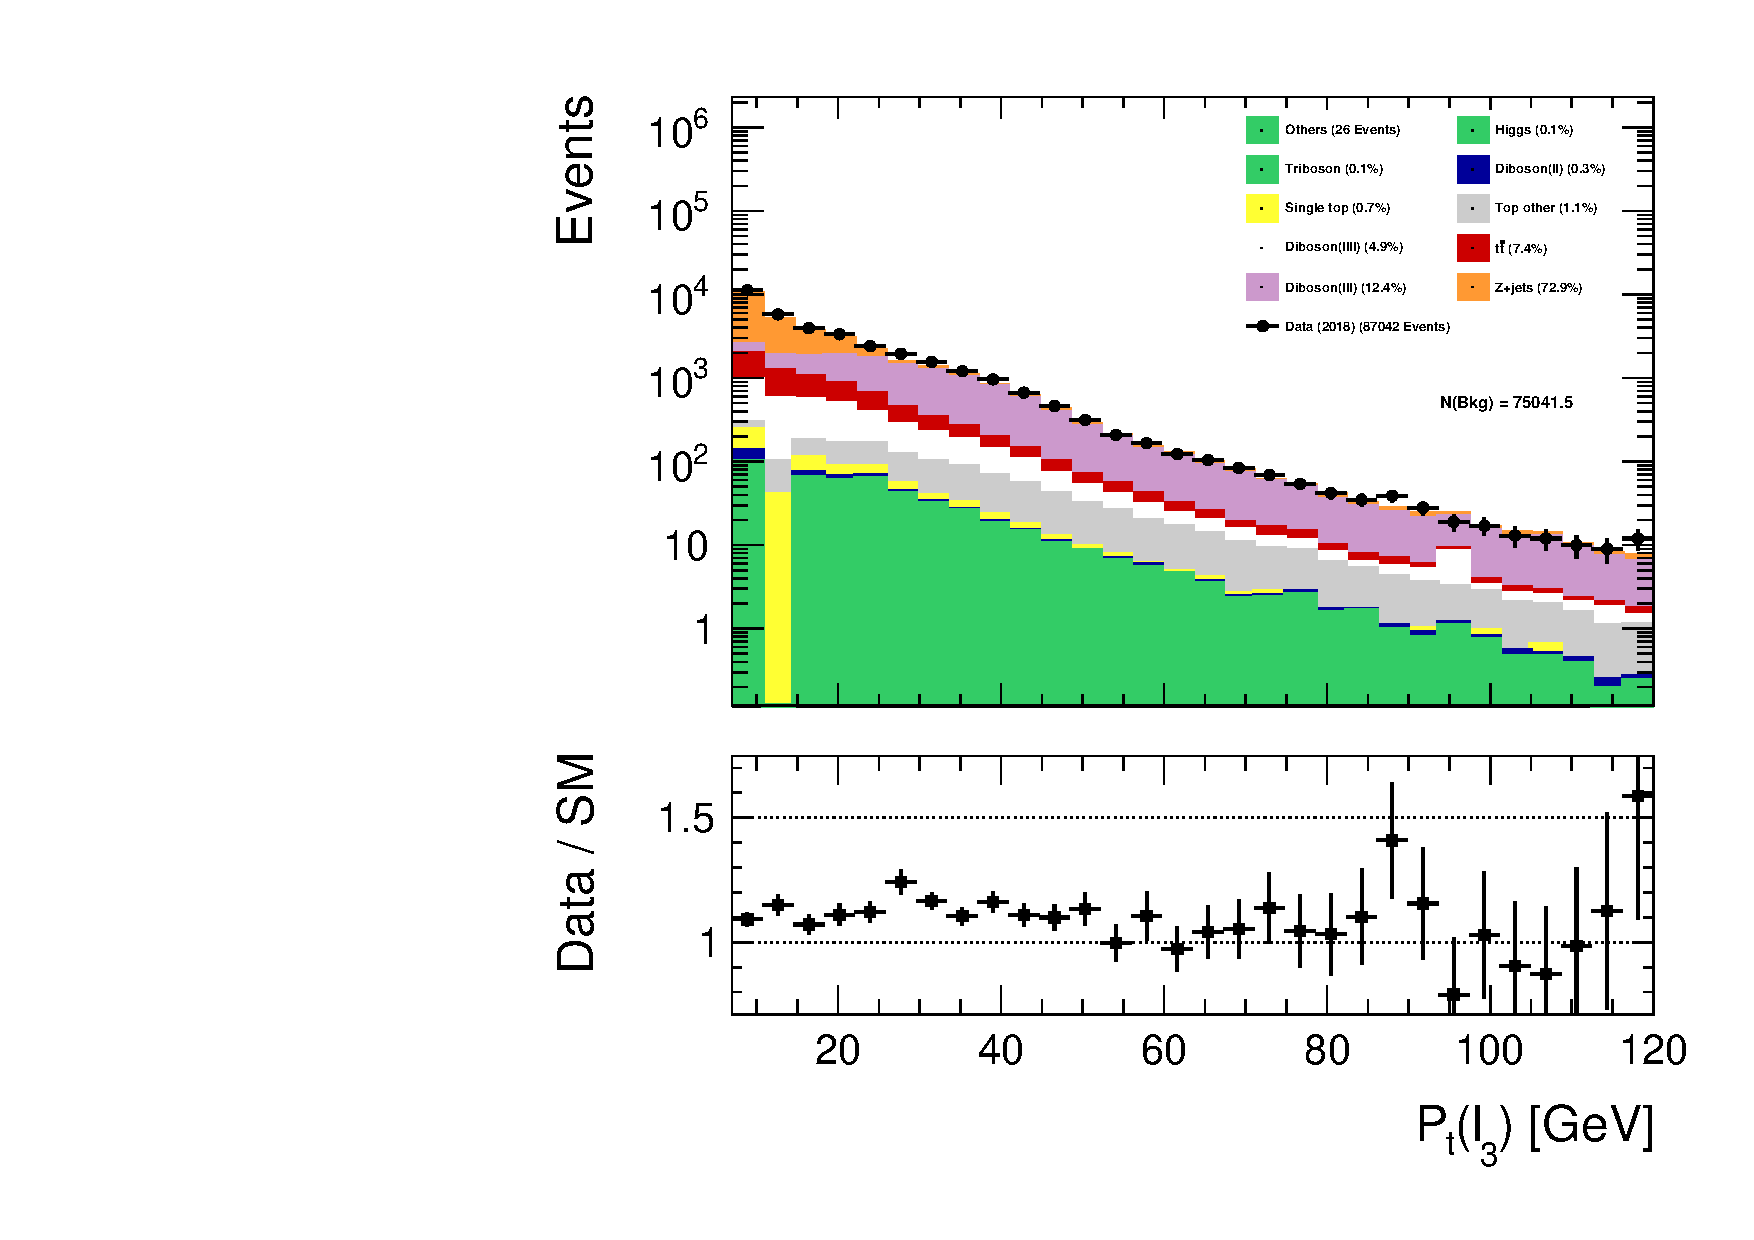
\includegraphics[width=\textwidth]{Figures/FeaturesHistograms/lep3_Pt.pdf}
        \caption{}
        \label{fig:lep3_Pt}
    \end{subfigure}
    \hfill
    \begin{subfigure}{.525\textwidth}
        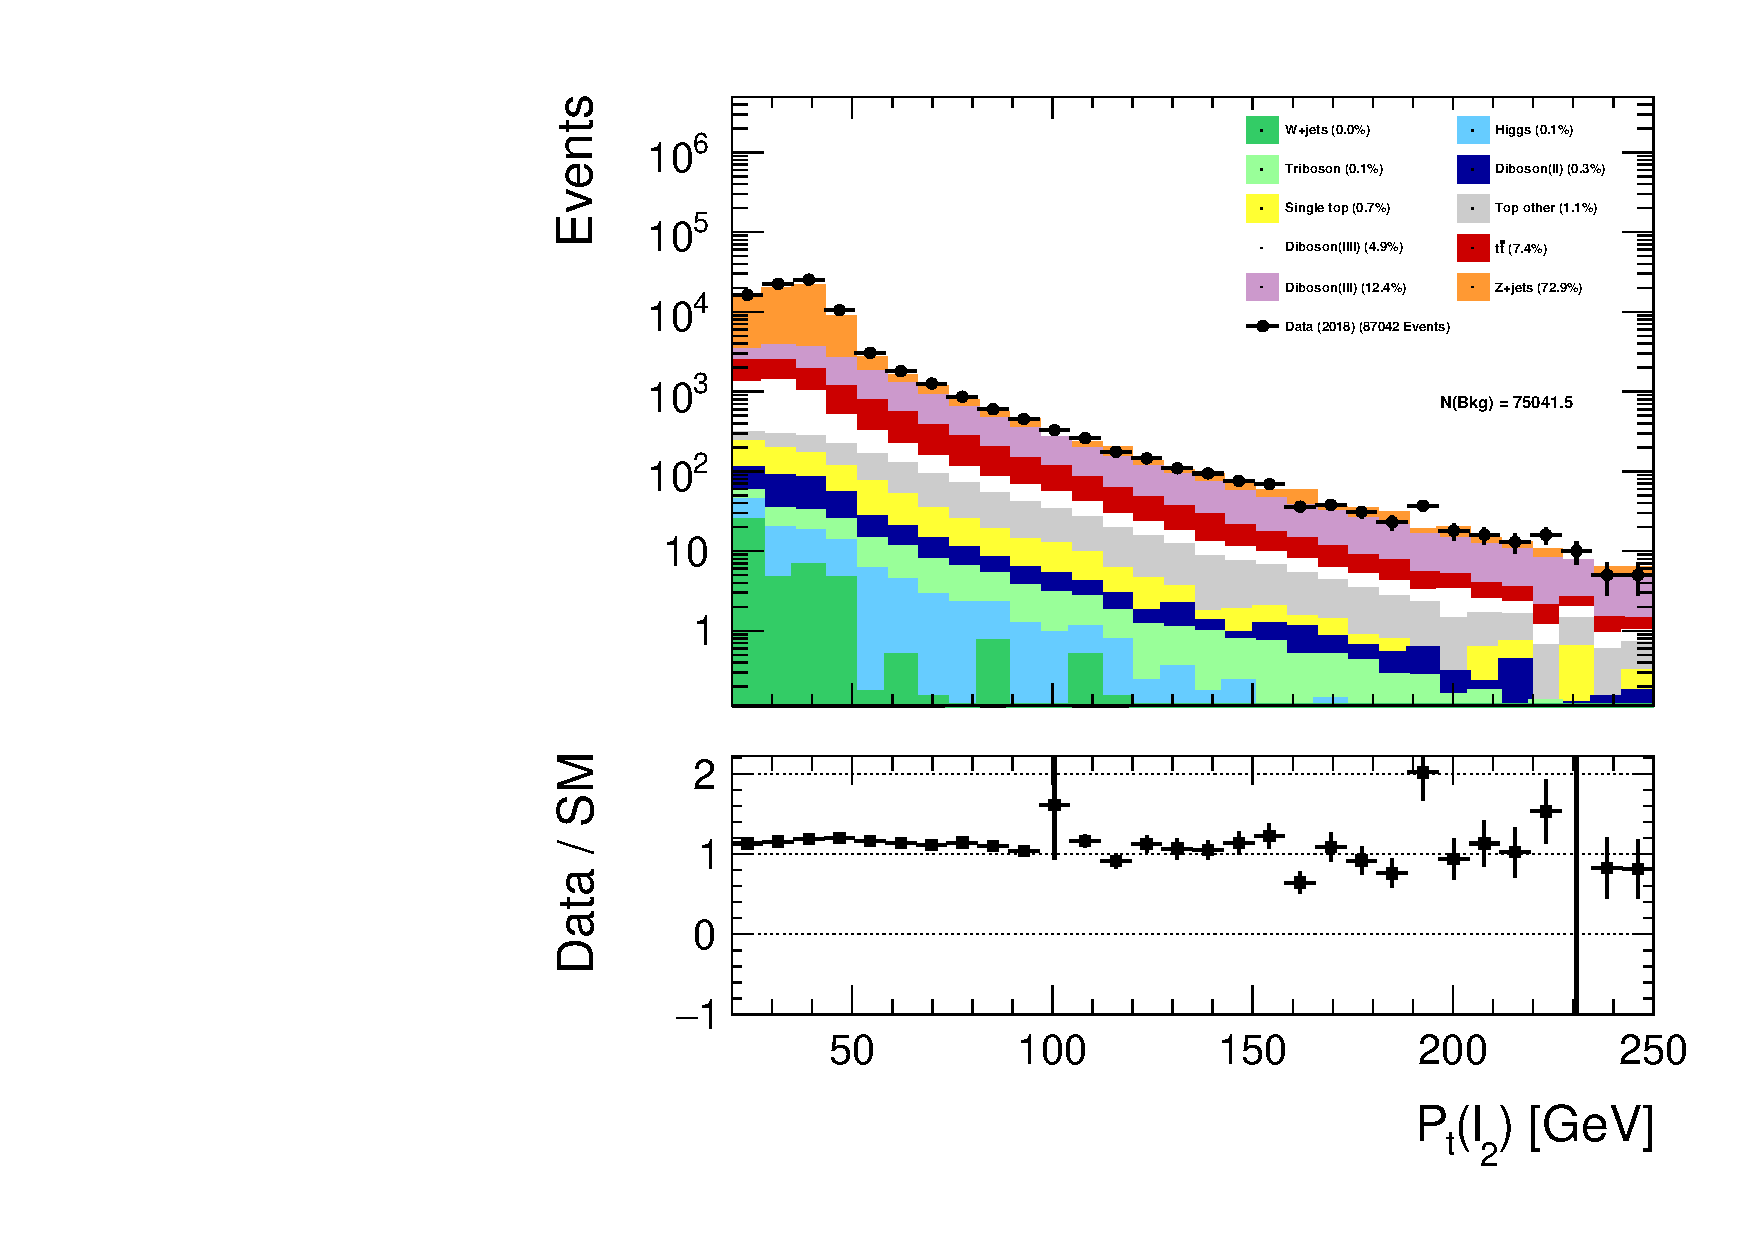
\includegraphics[width=\textwidth]{Figures/FeaturesHistograms/lep2_Pt.pdf}
        \caption{}
        \label{fig:lep2_Pt}
    \end{subfigure}
    }
    \makebox[0.95\linewidth][c]{%
    \begin{subfigure}{.405\textwidth}
        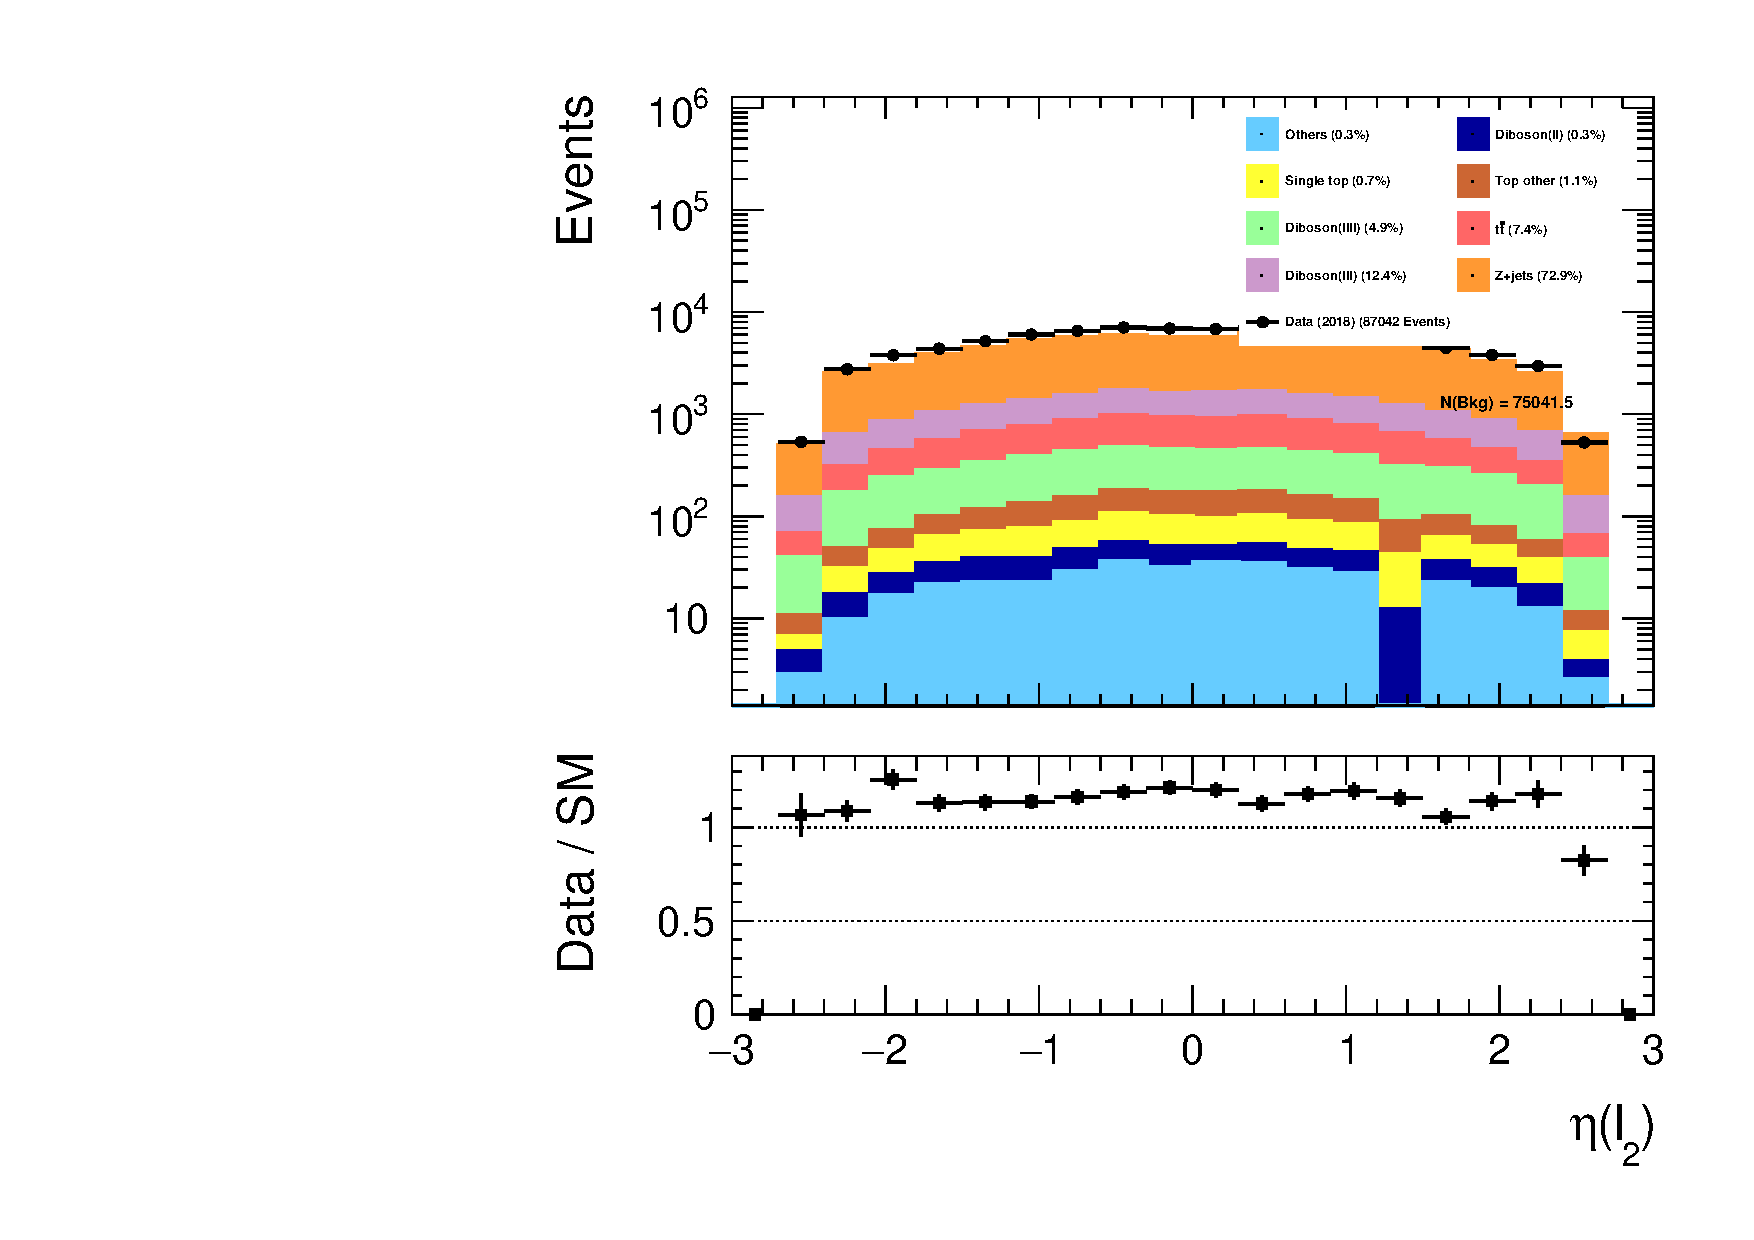
\includegraphics[width=\textwidth]{Figures/FeaturesHistograms/lep2_Eta.pdf}
        \caption{}
        \label{fig:lep2_Eta}
    \end{subfigure}
    \hfill
    \begin{subfigure}{.525\textwidth}
        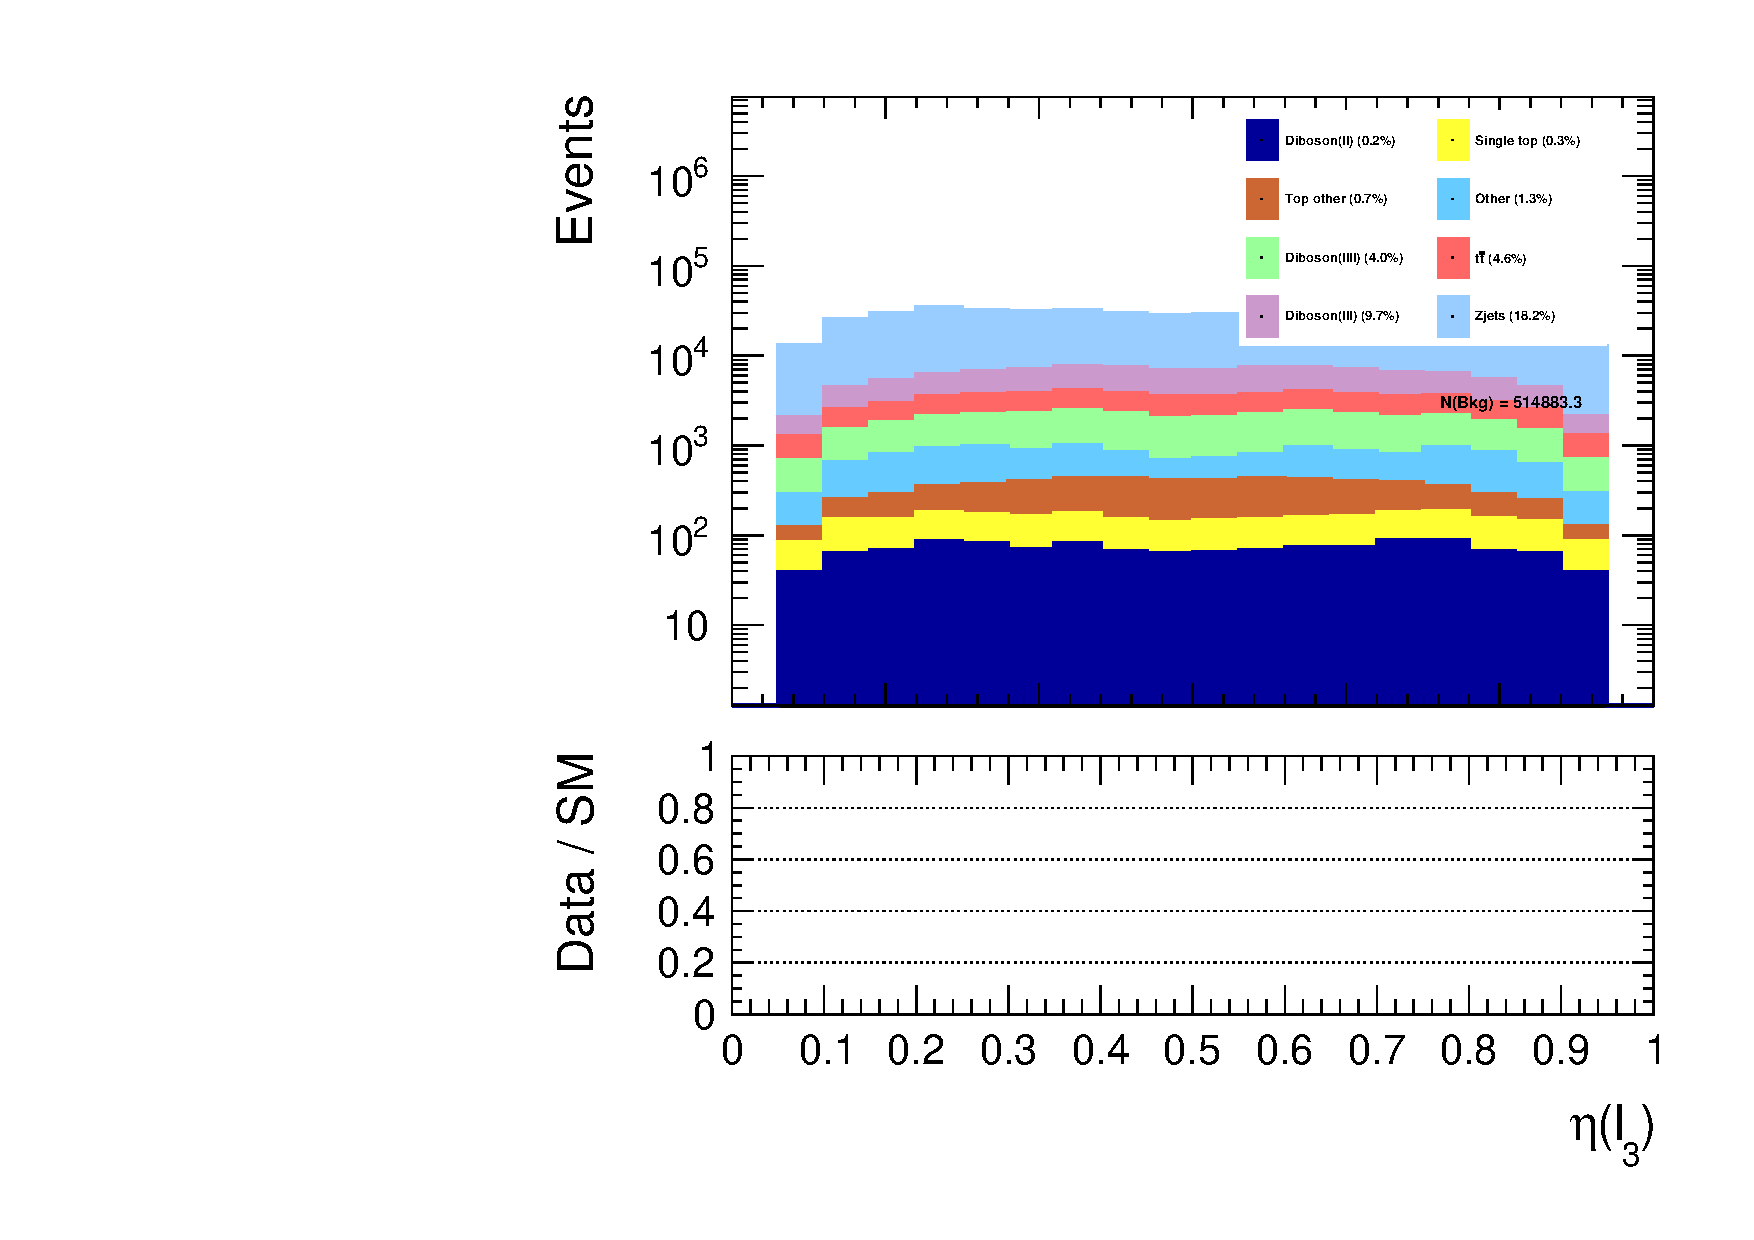
\includegraphics[width=\textwidth]{Figures/FeaturesHistograms/lep3_Eta.pdf}
        \caption{}
        \label{fig:lep3_Eta}
    \end{subfigure}
    }
    \caption[\ac{MC} simulated and measured data comparison and event distribution for each channel over $P_t$ for the first, 
    second and third lepton. Similarly, the distribution over $\eta$ for the first, second and third lepton.]{
        \ac{MC} simulated and measured data comparison and event distribution for each channel over $P_t$ for the third \ref{fig:lep3_Pt} 
        and second \ref{fig:lep2_Pt} lepton. Similarly, the distribution over $\eta$ for the 
        second \ref{fig:lep2_Eta} and third \ref{fig:lep3_Eta} lepton.}
        \label{fig:Dist2}
    \end{figure}
    \newpage
    \begin{figure}[H]
    \makebox[0.95\linewidth][c]{%
    \centering
    \begin{subfigure}{.405\textwidth}
        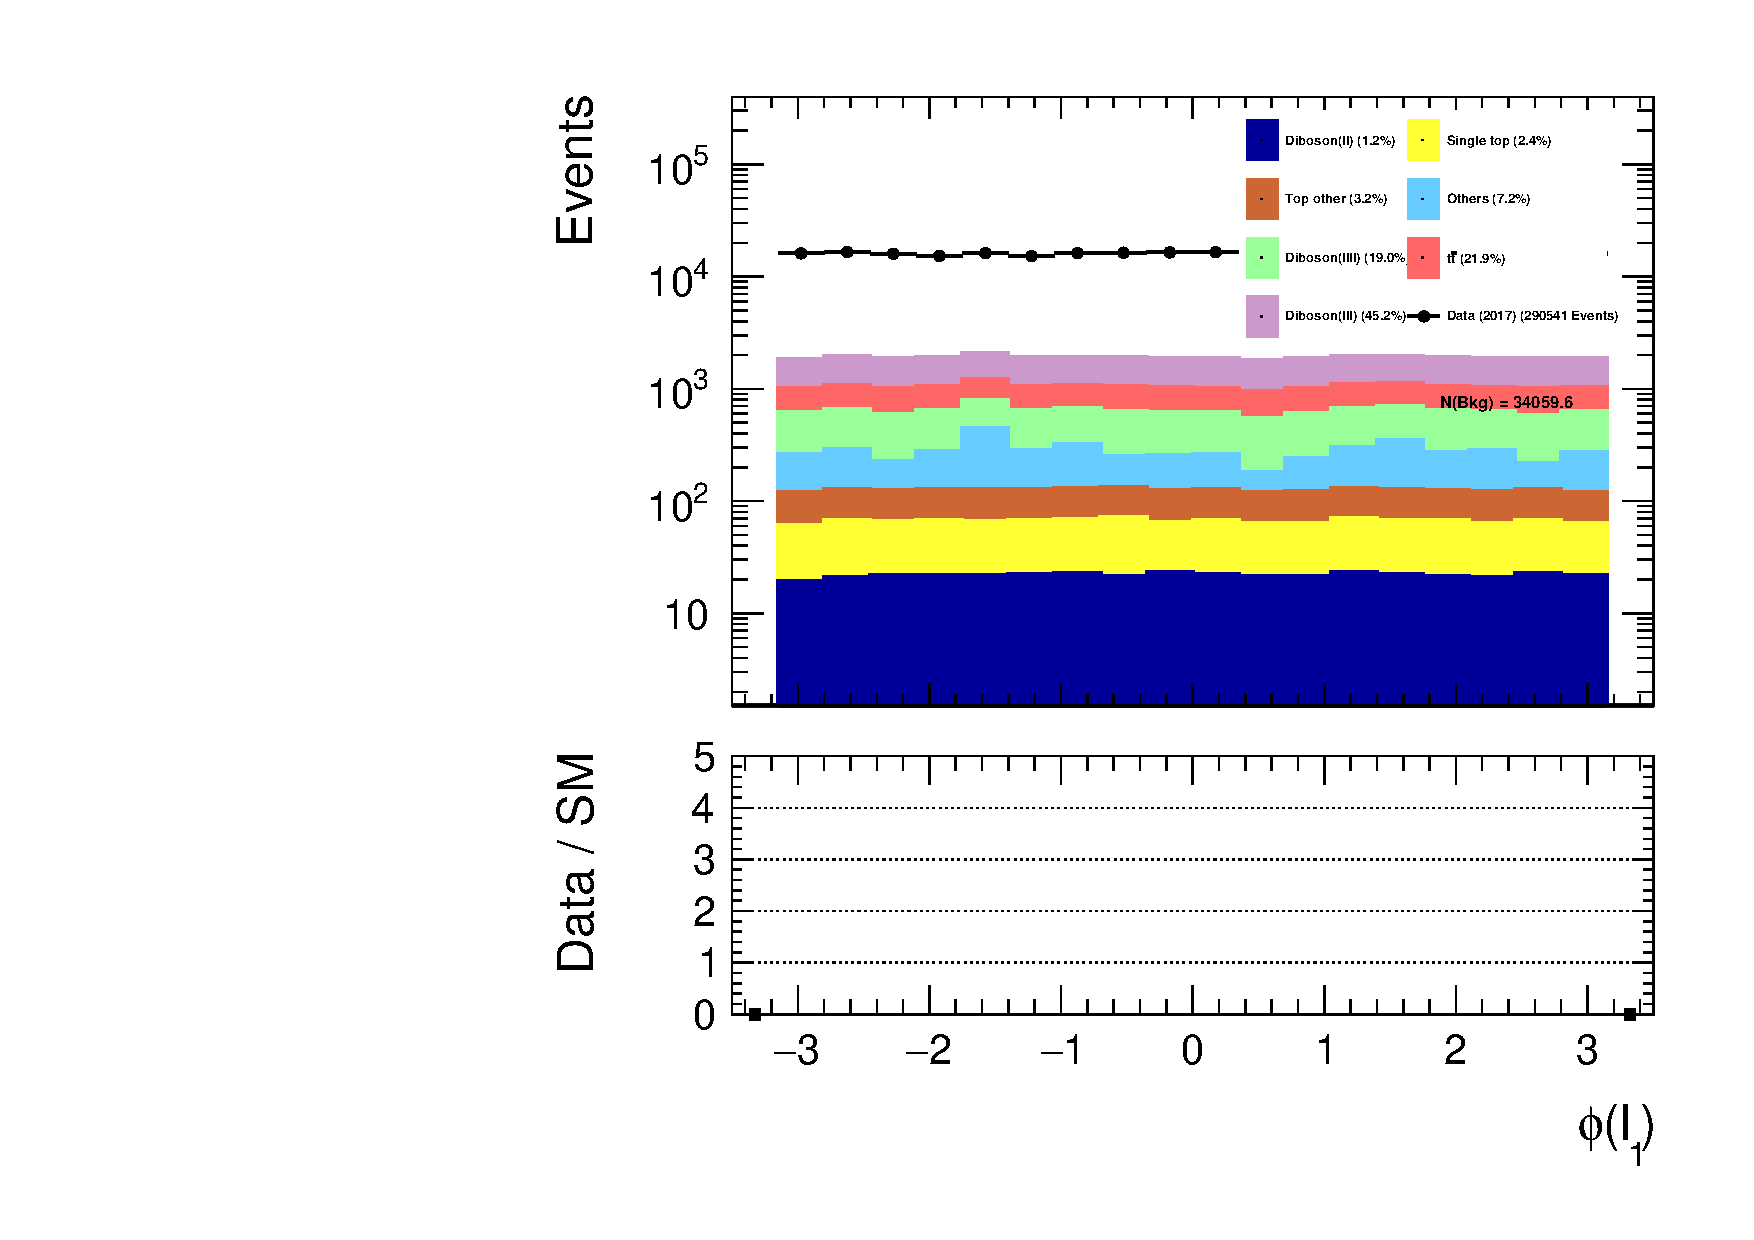
\includegraphics[width=\textwidth]{Figures/FeaturesHistograms/lep1_Phi.pdf}
        \caption{}
        \label{fig:lep1_Phi}
    \end{subfigure}
    \hfill
    \begin{subfigure}{.525\textwidth}
        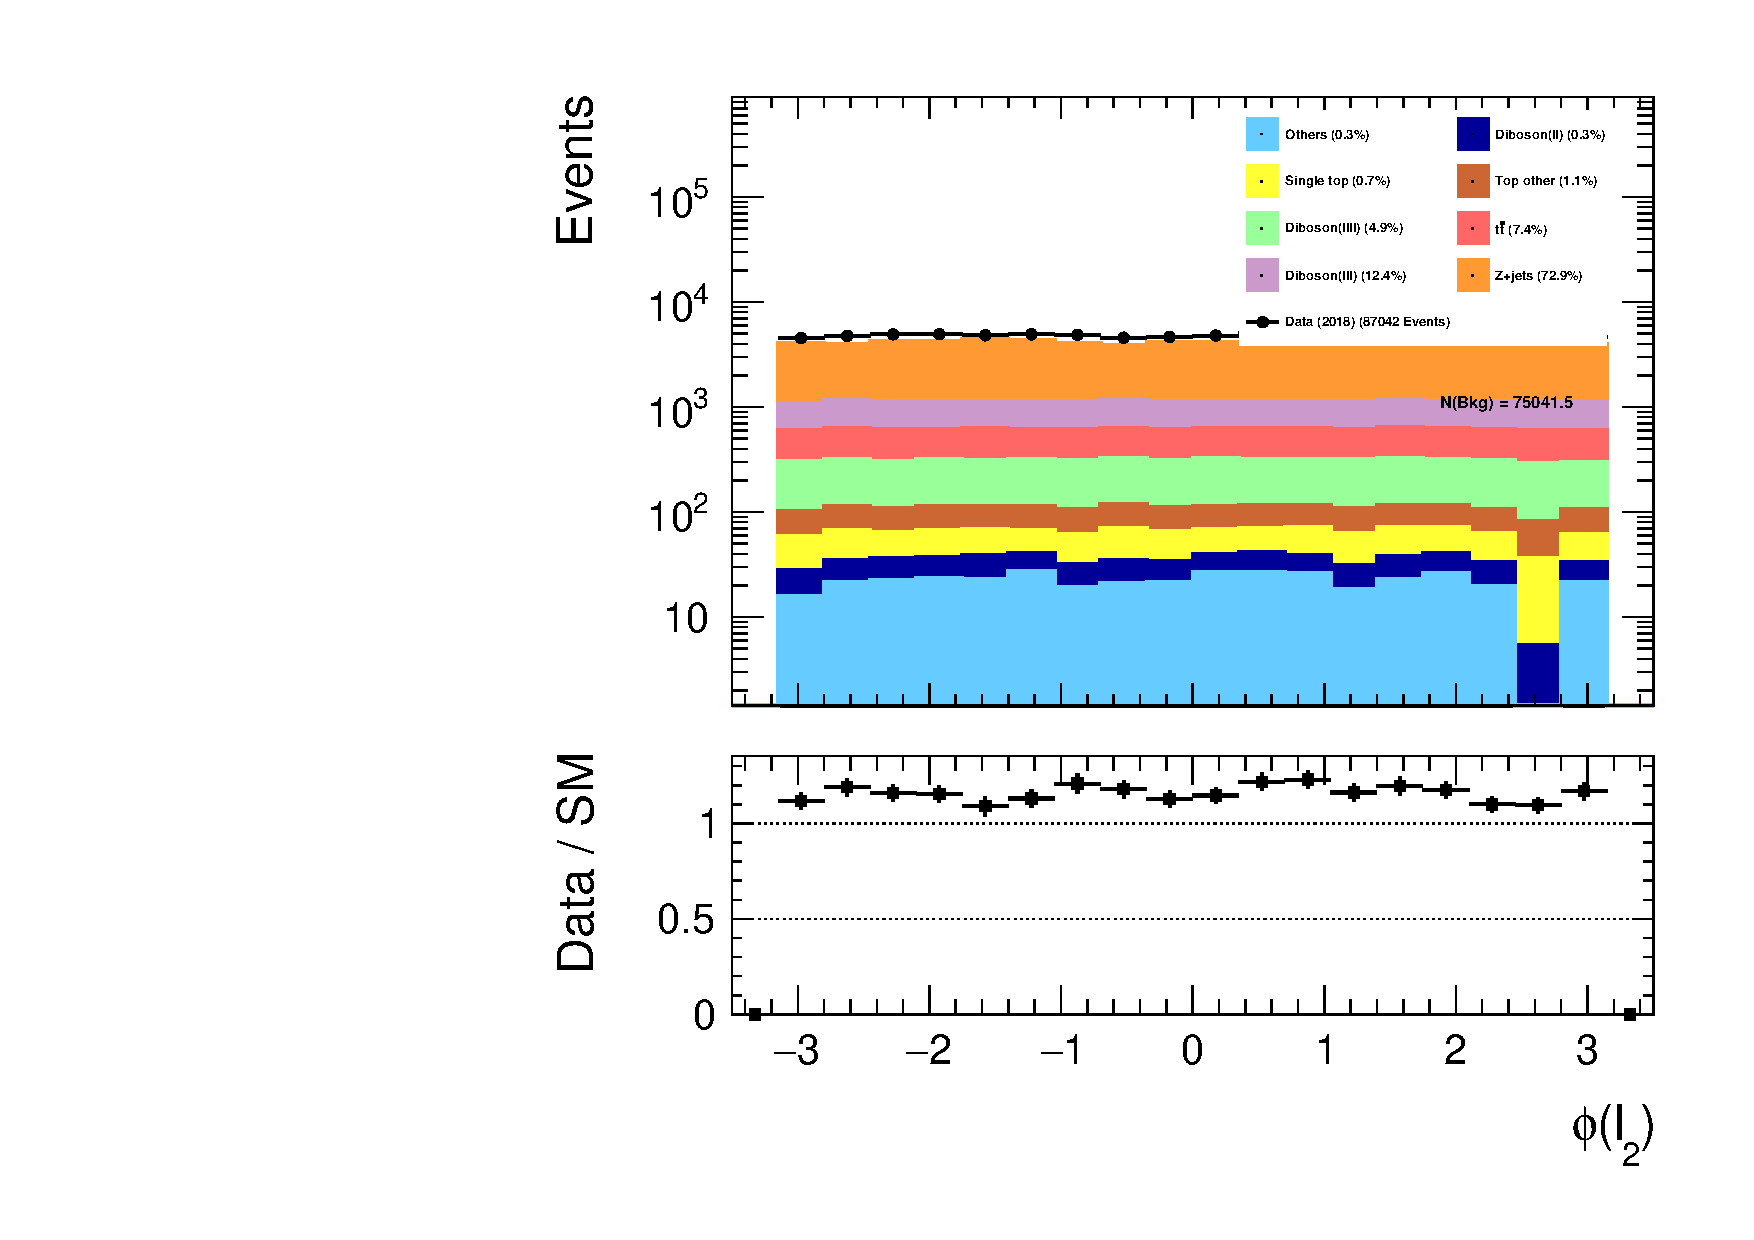
\includegraphics[width=\textwidth]{Figures/FeaturesHistograms/lep2_Phi.pdf}
        \caption{}
        \label{fig:lep2_Phi}
    \end{subfigure}
    }
    \makebox[0.95\linewidth][c]{%
    \begin{subfigure}{.405\textwidth}
        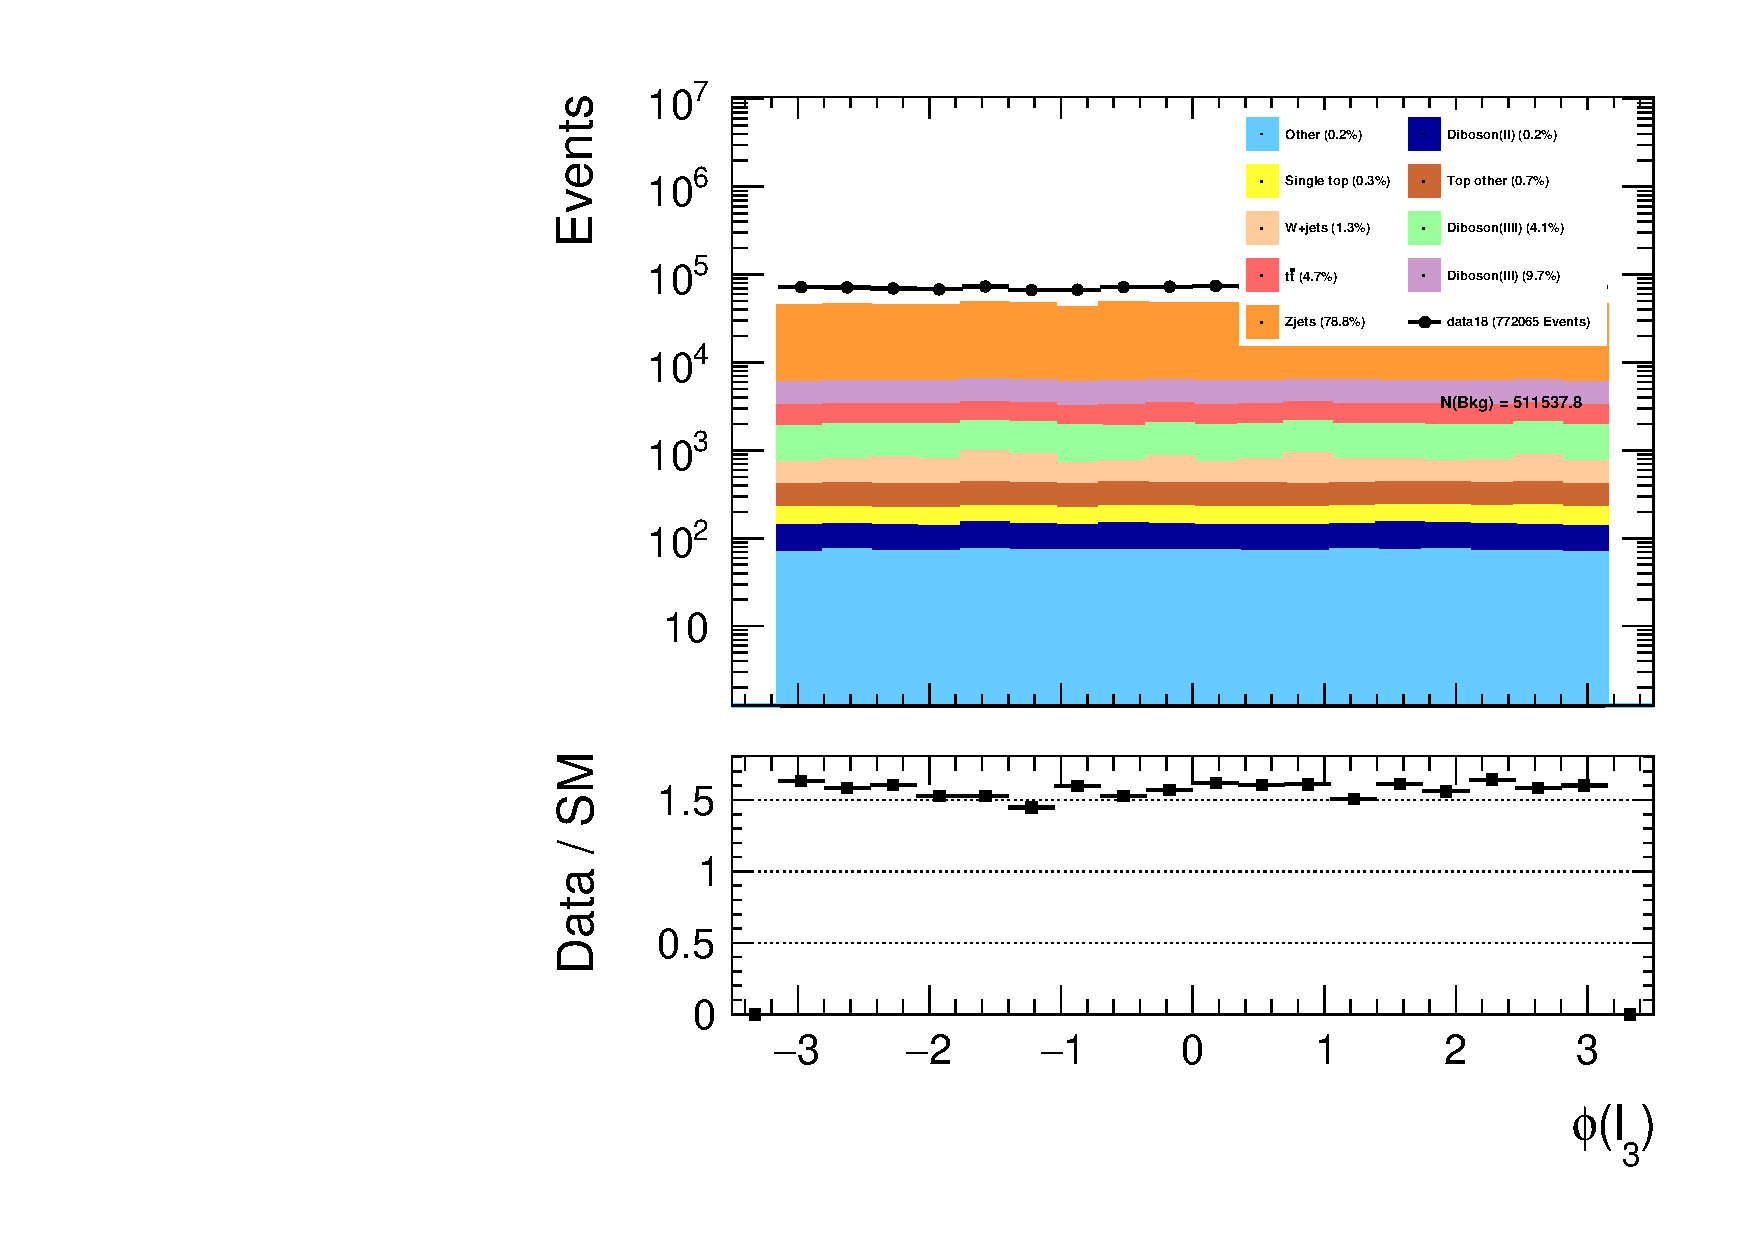
\includegraphics[width=\textwidth]{Figures/FeaturesHistograms/lep3_Phi.pdf}
        \caption{}
        \label{fig:lep3_Phi}
    \end{subfigure}
    \hfill
    \begin{subfigure}{.525\textwidth}
        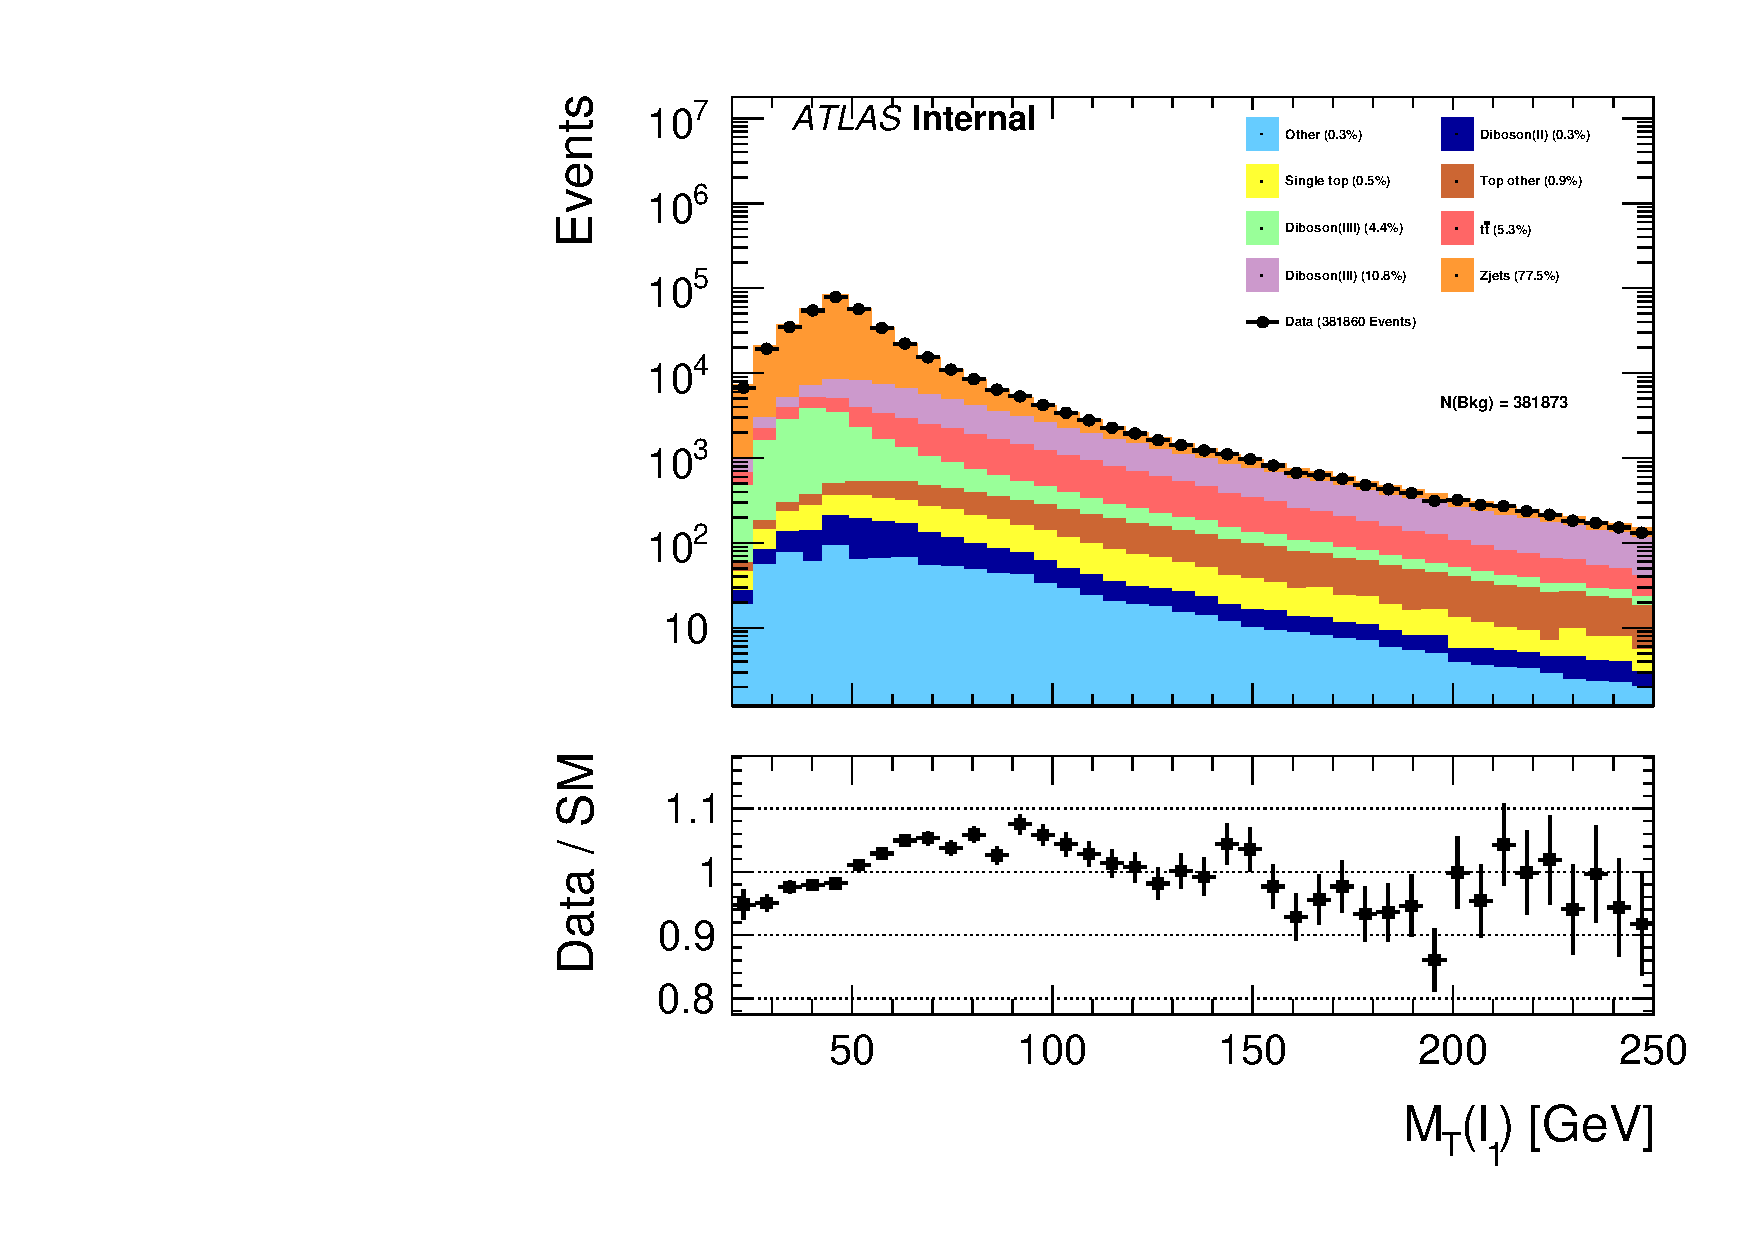
\includegraphics[width=\textwidth]{Figures/FeaturesHistograms/lep1_Mt.pdf}
        \caption{}
        \label{fig:lep1_Mt}
    \end{subfigure}
    }
    \makebox[0.95\linewidth][c]{%
    \begin{subfigure}{.405\textwidth}
        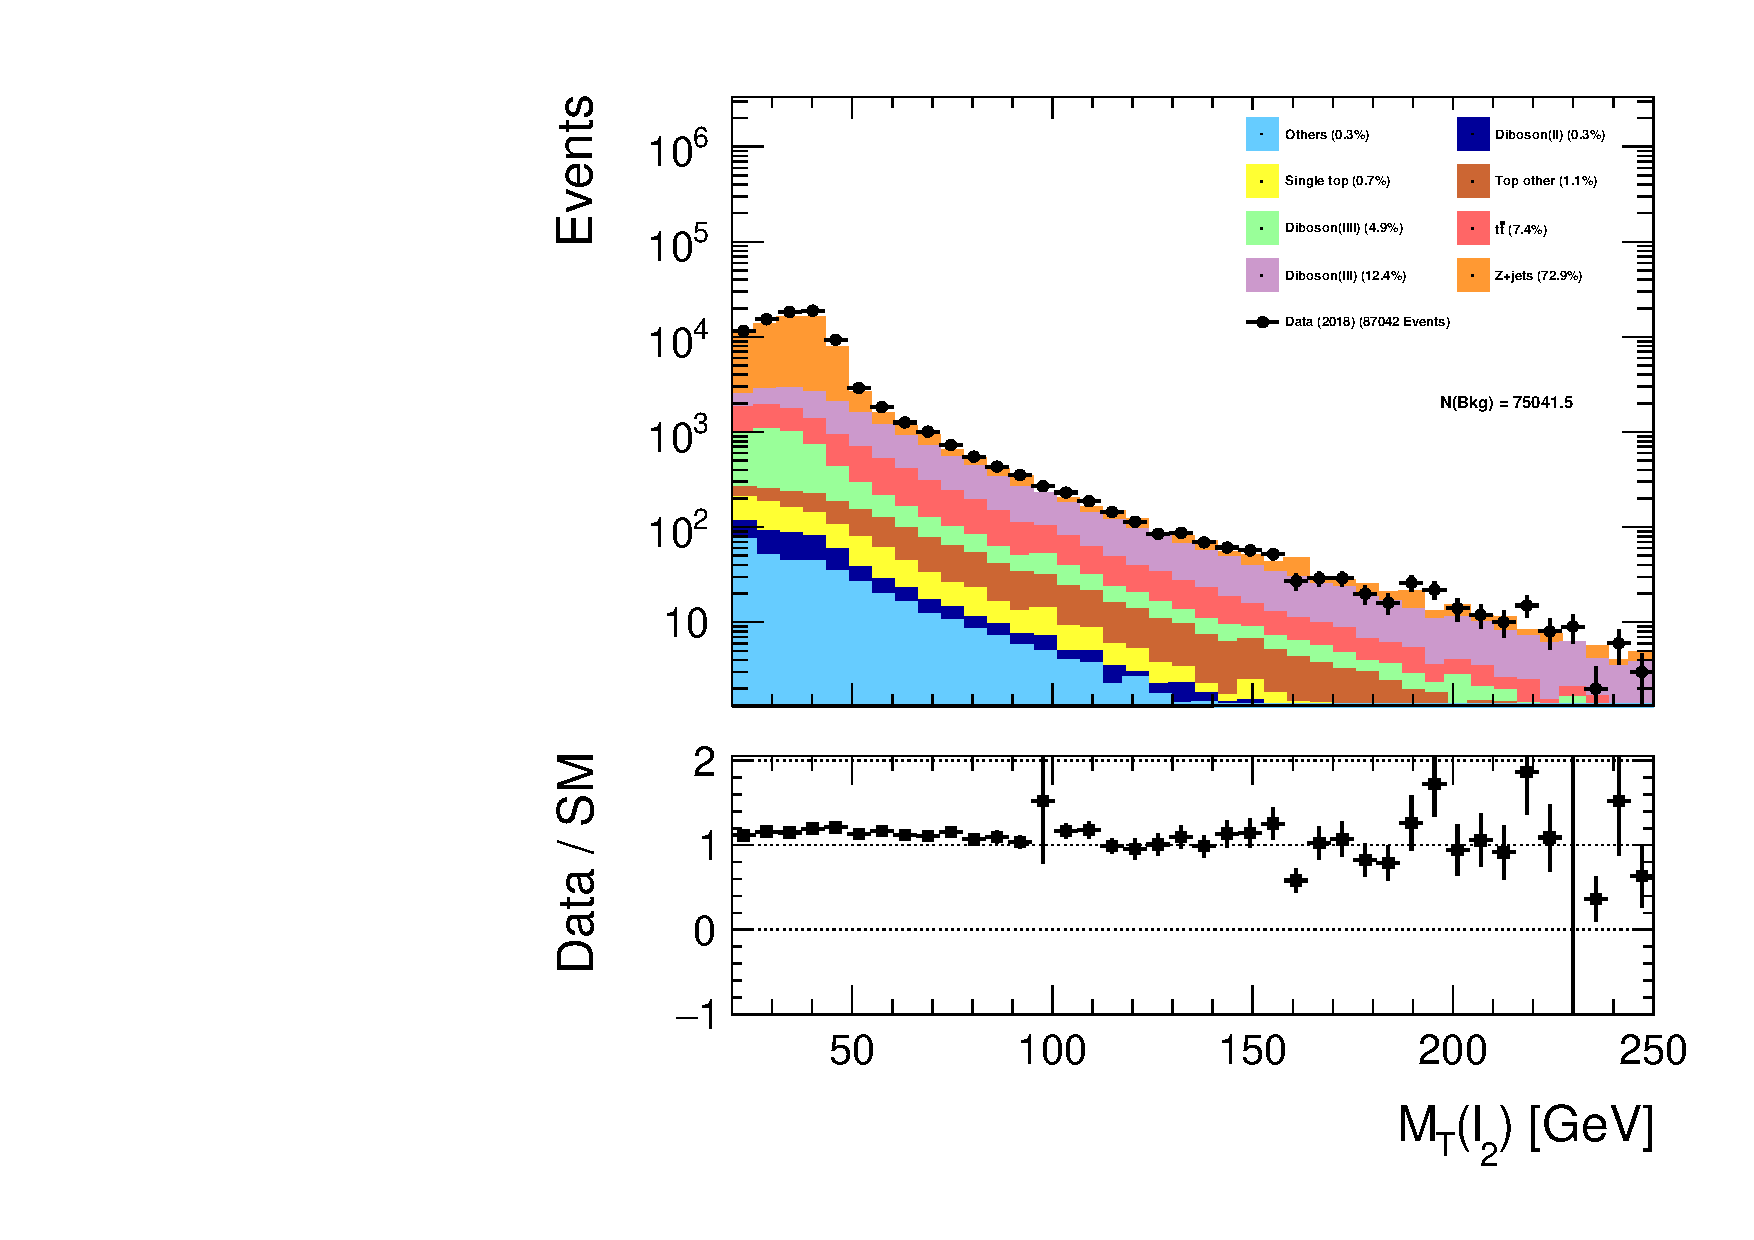
\includegraphics[width=\textwidth]{Figures/FeaturesHistograms/lep2_Mt.pdf}
        \caption{}
        \label{fig:lep2_Mt}
    \end{subfigure}
    \hfill
    \begin{subfigure}{.525\textwidth}
        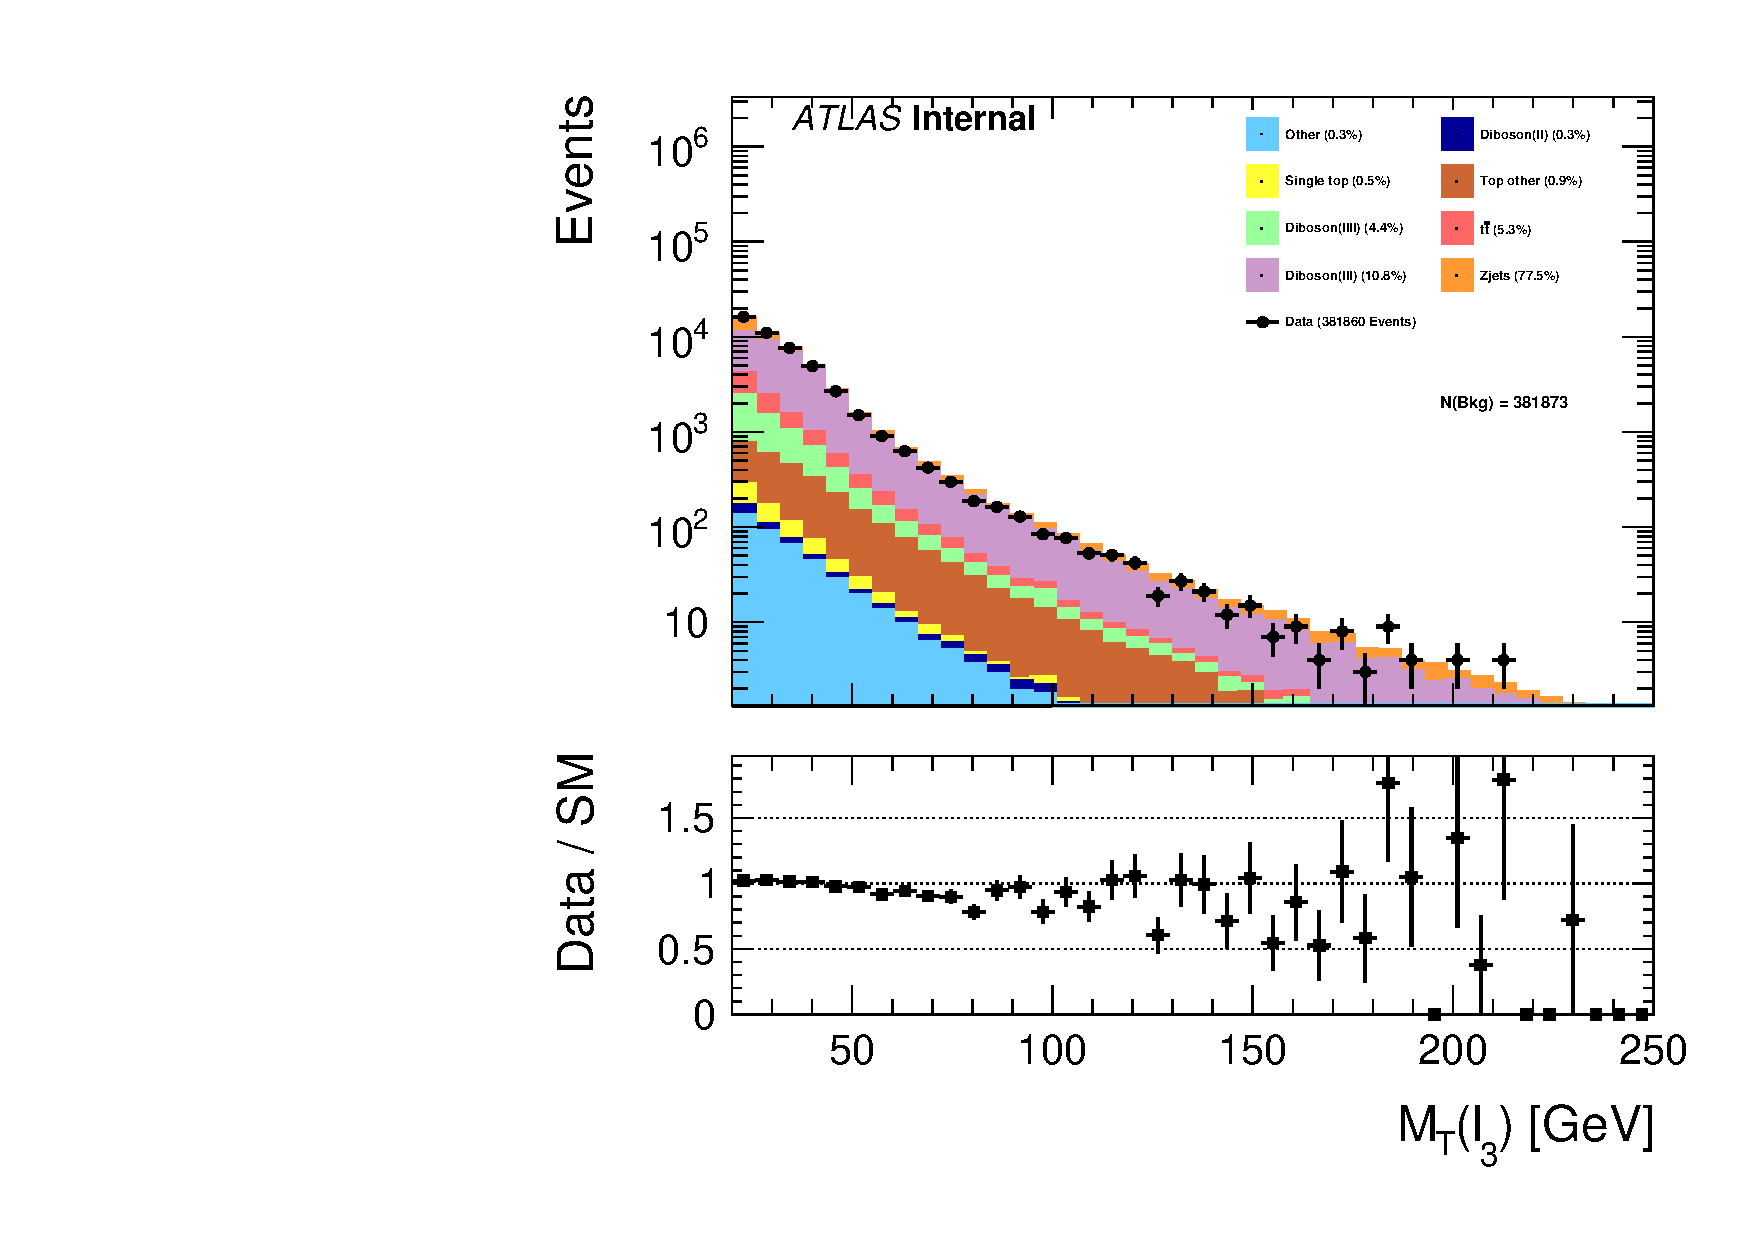
\includegraphics[width=\textwidth]{Figures/FeaturesHistograms/lep3_Mt.pdf}
        \caption{}
        \label{fig:lep3_Mt}
    \end{subfigure}
    }
    \caption[\ac{MC} simulated and measured data comparison and event distribution for each channel over $\phi$ for the first, 
    second and third lepton. Similarly, the distribution over $m_t$ for the first, second and third lepton.]{\ac{MC} simulated and measured data 
    comparison and event distribution for each channel over $\phi$ for the first \ref{fig:lep1_Phi}, 
    second \ref{fig:lep2_Phi} and third \ref{fig:lep3_Phi} lepton. Similarly, the distribution over $m_t$
    for the first \ref{fig:lep1_Mt}, second \ref{fig:lep2_Mt} and third \ref{fig:lep3_Mt} lepton.}
\end{figure}
\newpage
\begin{figure}[H]
    \makebox[0.95\linewidth][c]{%
    \centering
    \begin{subfigure}{.405\textwidth}
        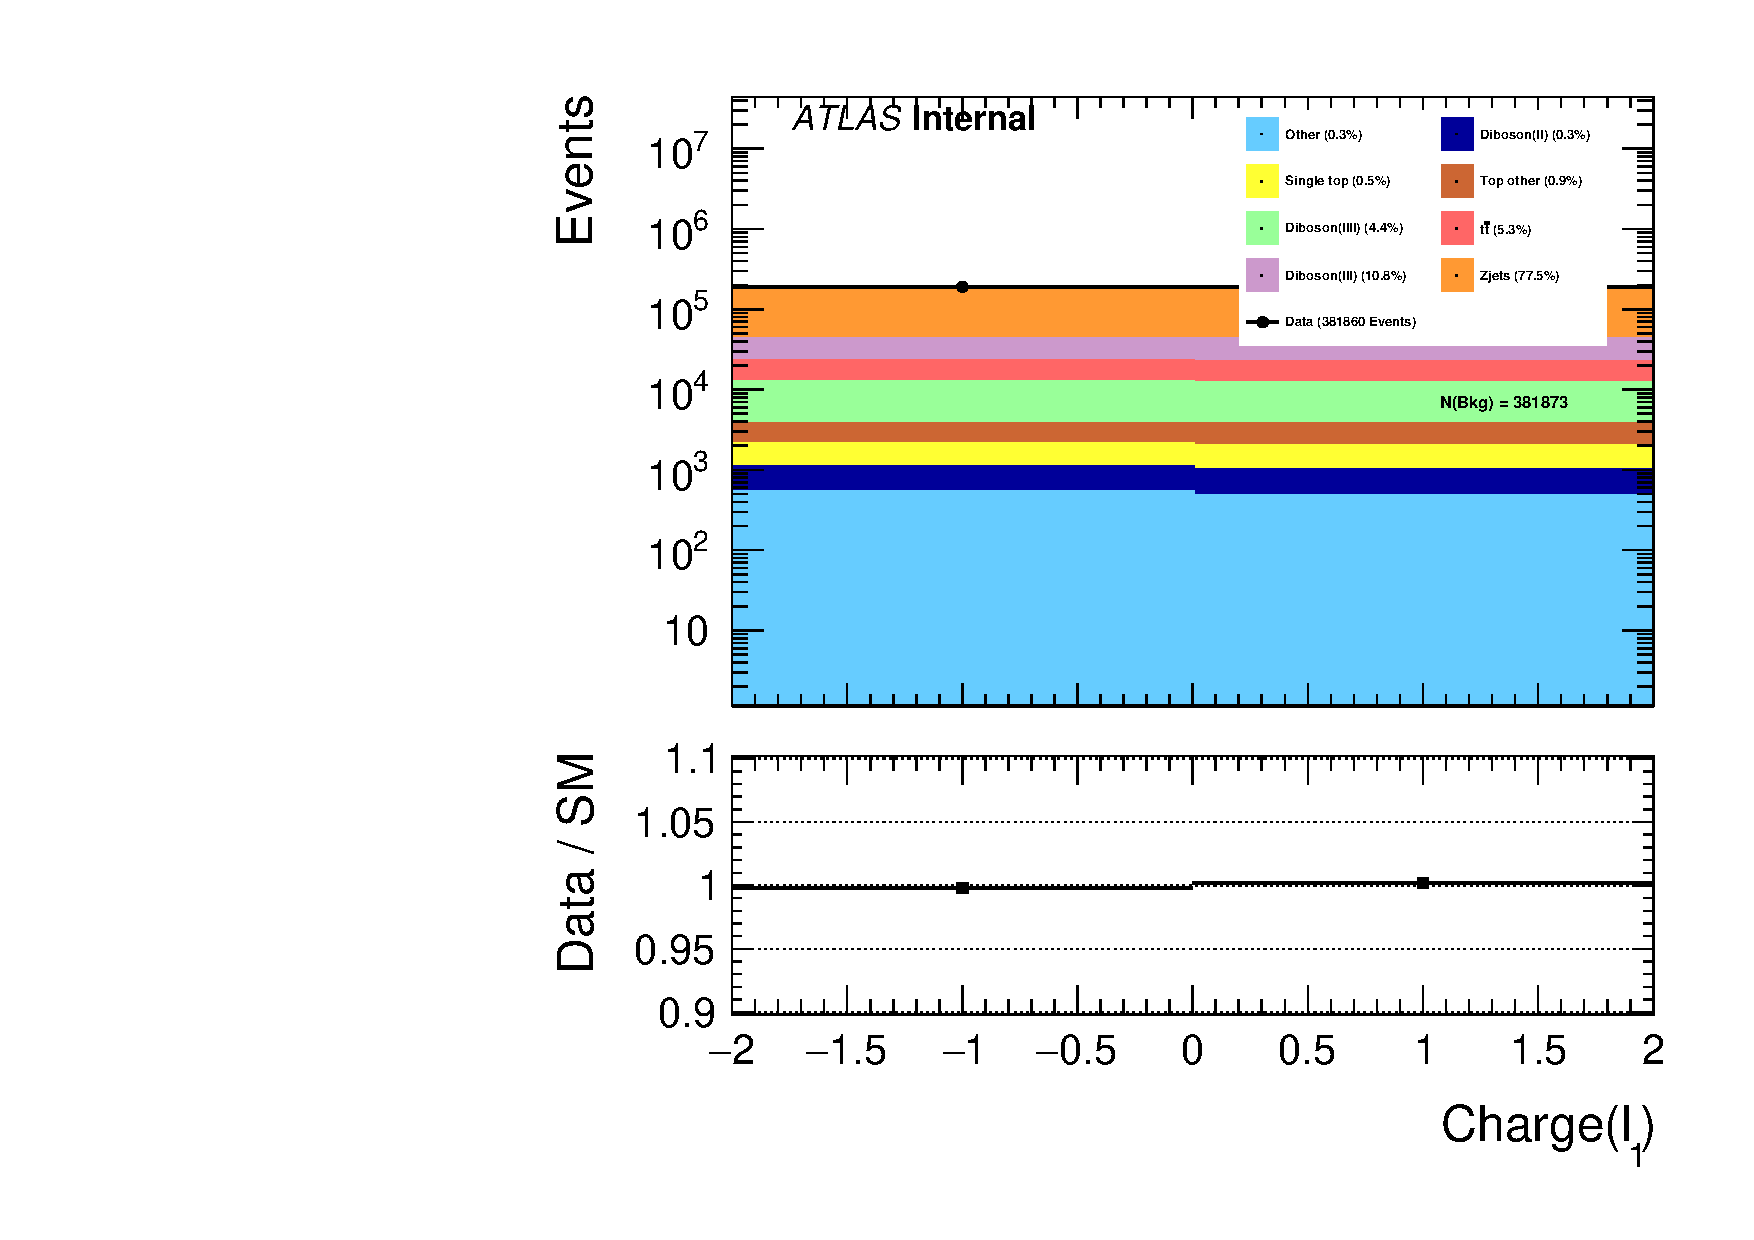
\includegraphics[width=\textwidth]{Figures/FeaturesHistograms/lep1_Charge.pdf}
        \caption{}
        \label{fig:lep1_Charge}
    \end{subfigure}
    \hfill
    \begin{subfigure}{.525\textwidth}
        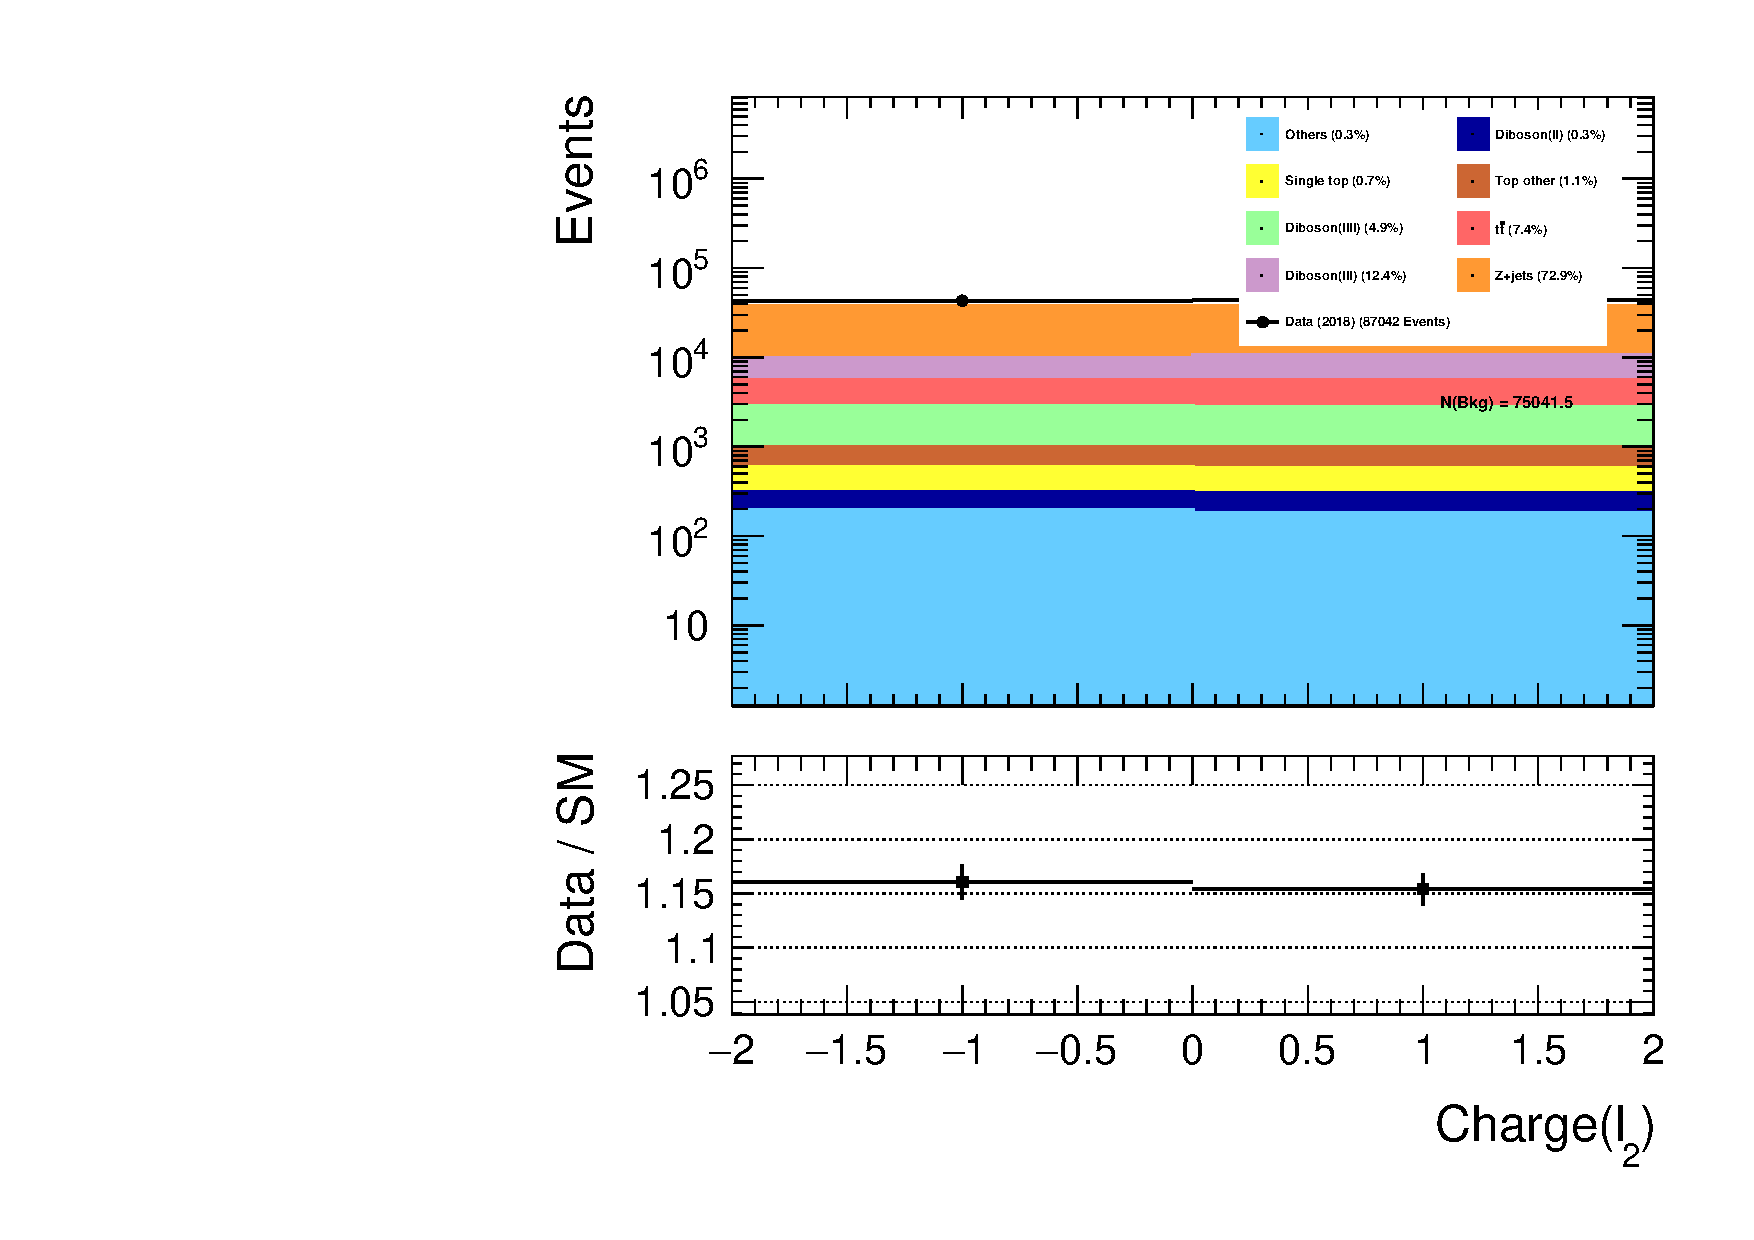
\includegraphics[width=\textwidth]{Figures/FeaturesHistograms/lep2_Charge.pdf}
        \caption{}
        \label{fig:lep2_Charge}
    \end{subfigure}
    }
    \makebox[0.95\linewidth][c]{%
    \begin{subfigure}{.405\textwidth}
        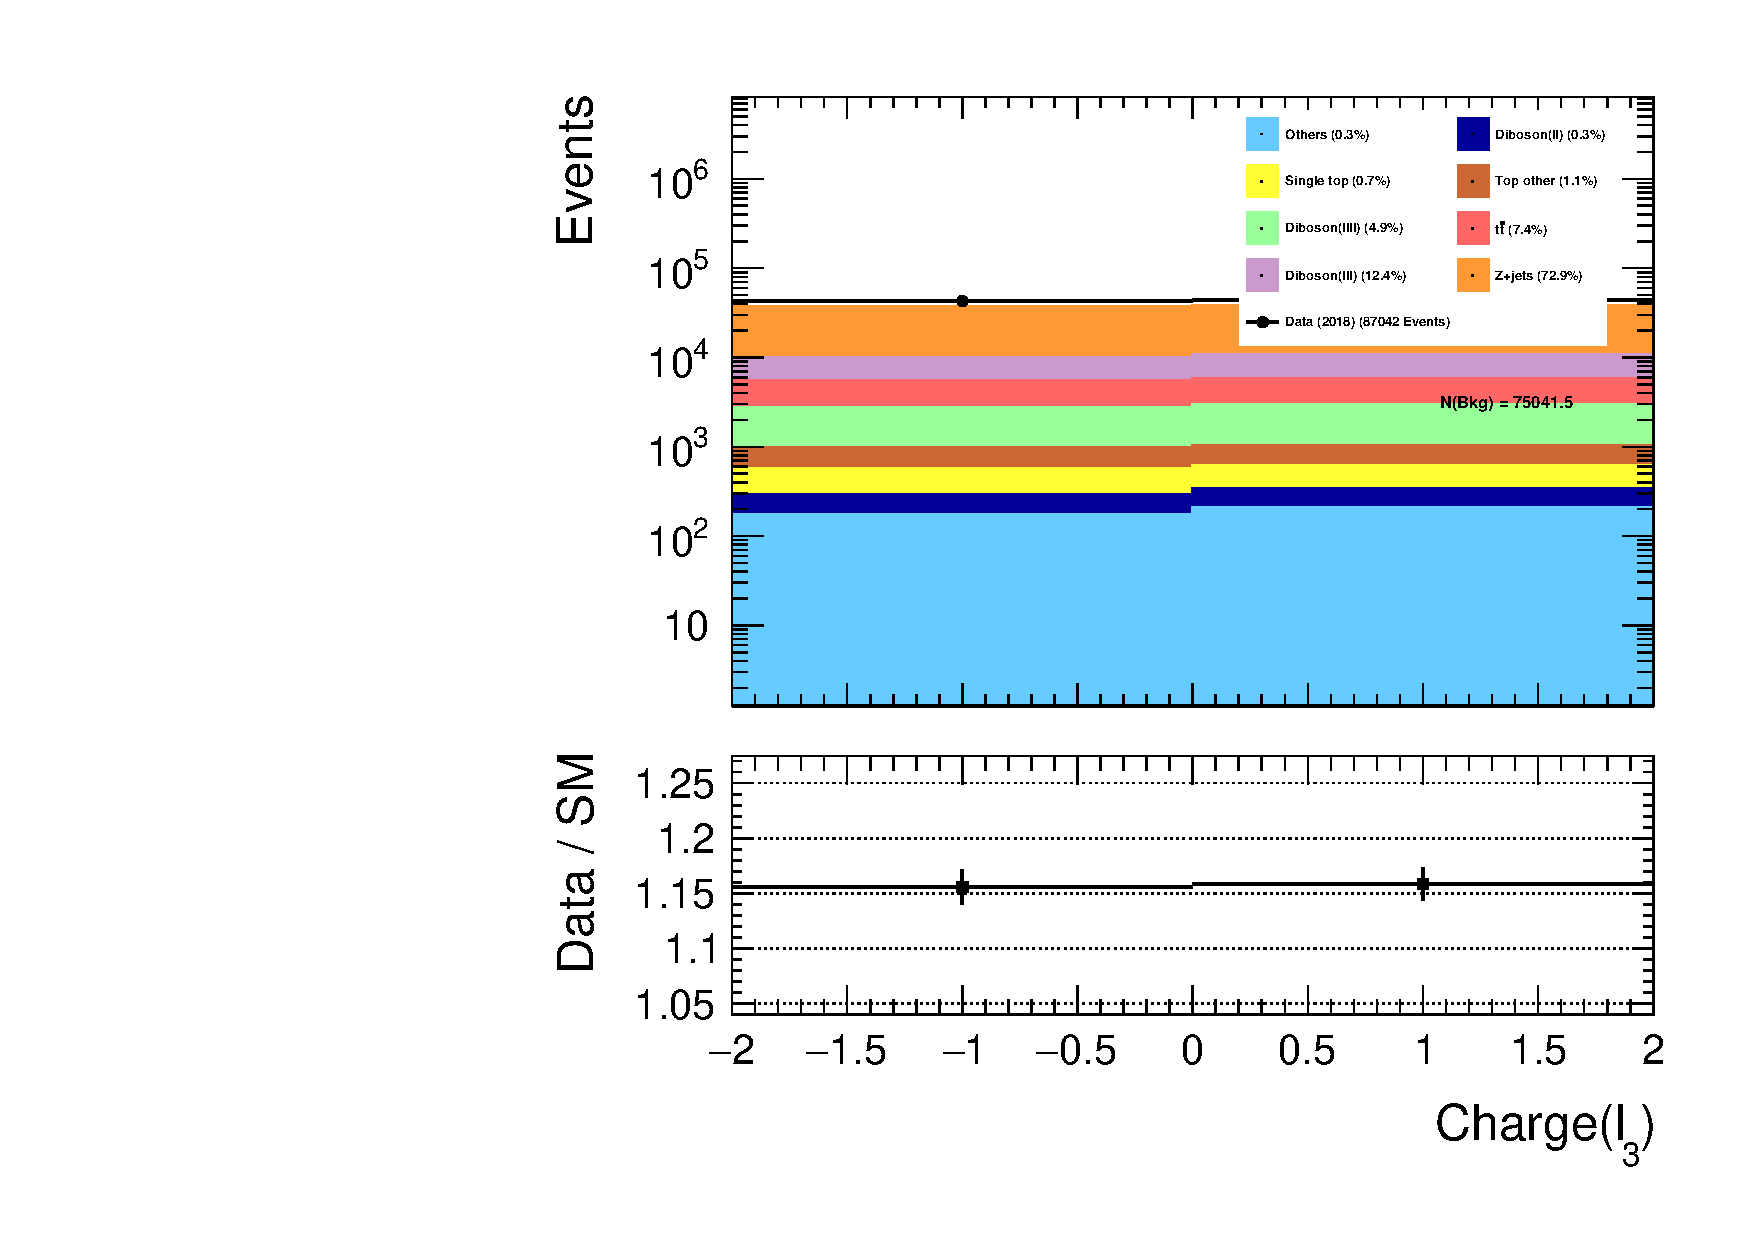
\includegraphics[width=\textwidth]{Figures/FeaturesHistograms/lep3_Charge.pdf}
        \caption{}
        \label{fig:lep3_Charge}
    \end{subfigure}
    \hfill
    \begin{subfigure}{.525\textwidth}
        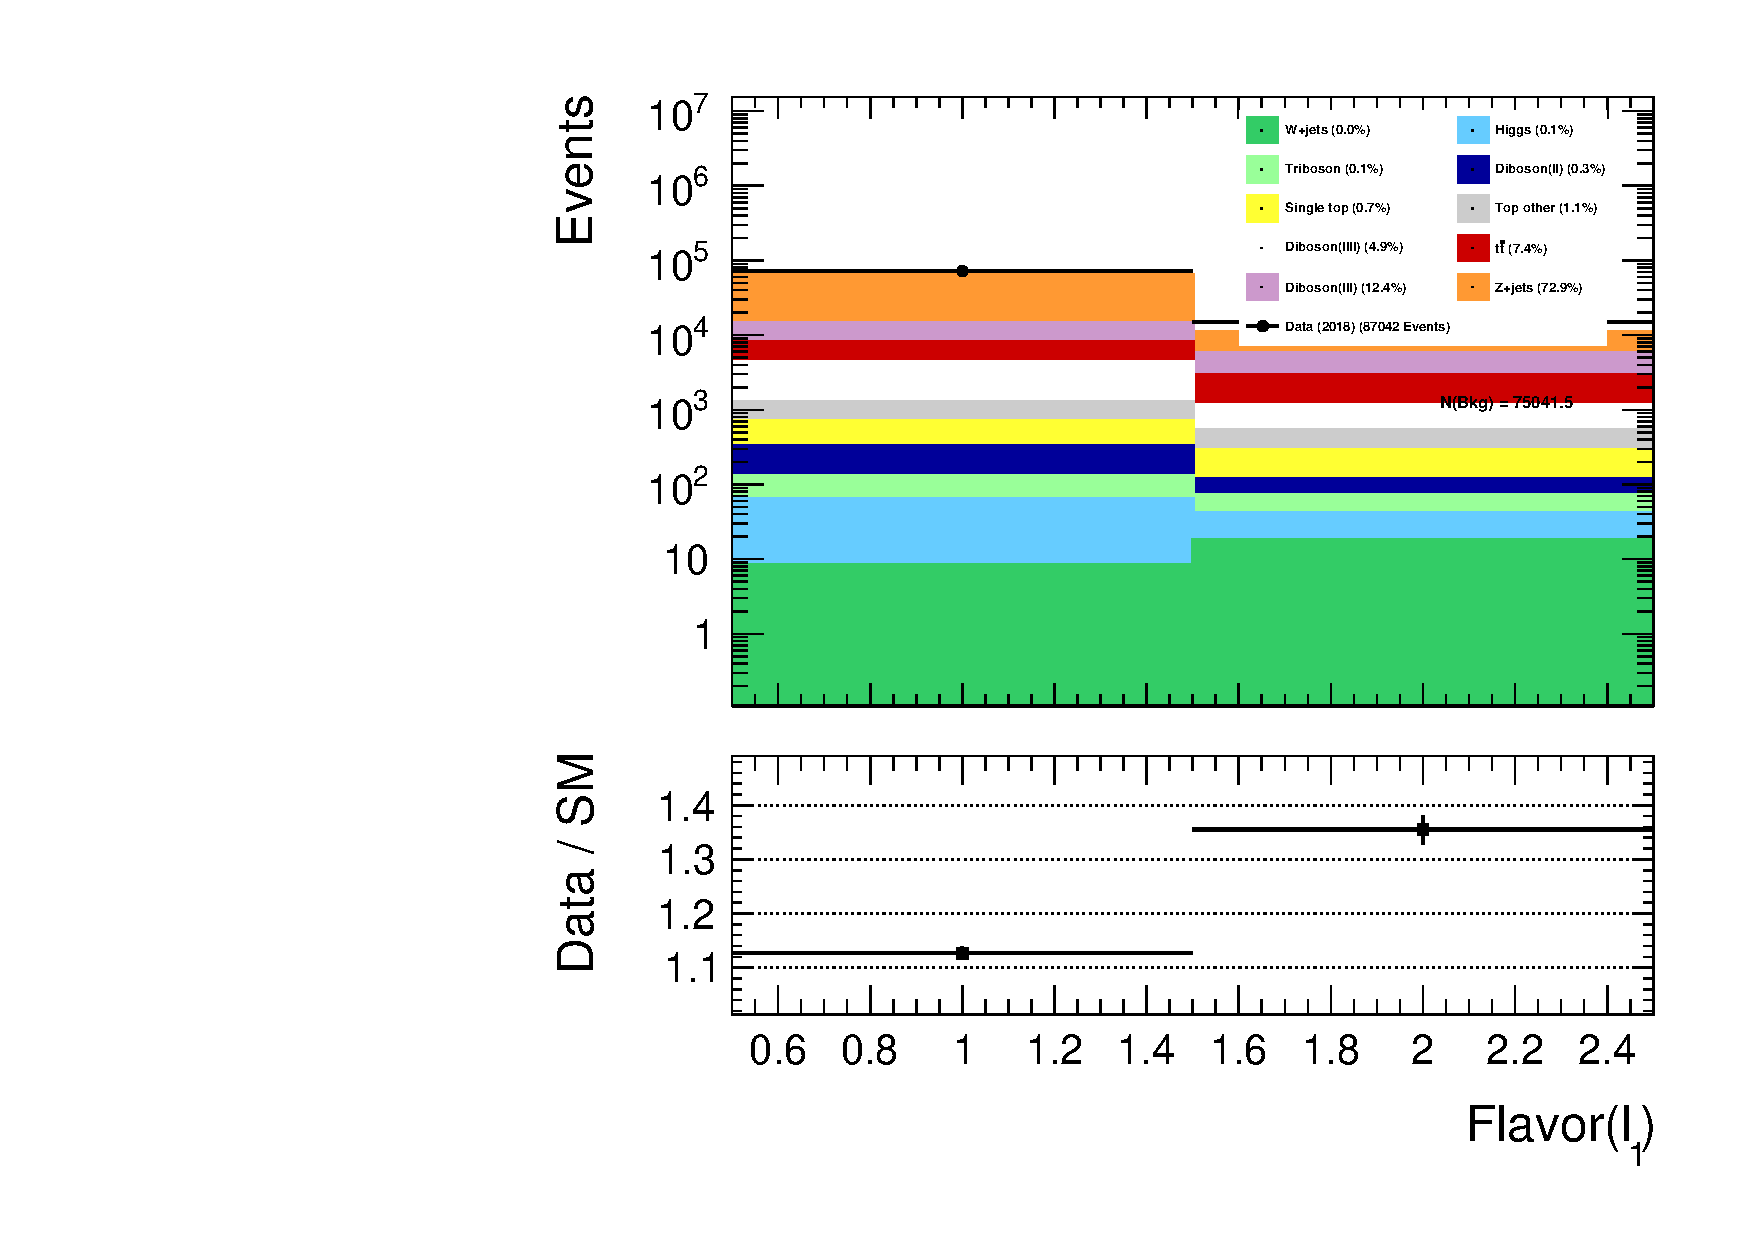
\includegraphics[width=\textwidth]{Figures/FeaturesHistograms/lep1_Flavor.pdf}
        \caption{}
        \label{fig:lep1_Flavor}
    \end{subfigure}
    }
    \makebox[0.95\linewidth][c]{%
    \begin{subfigure}{.405\textwidth}
        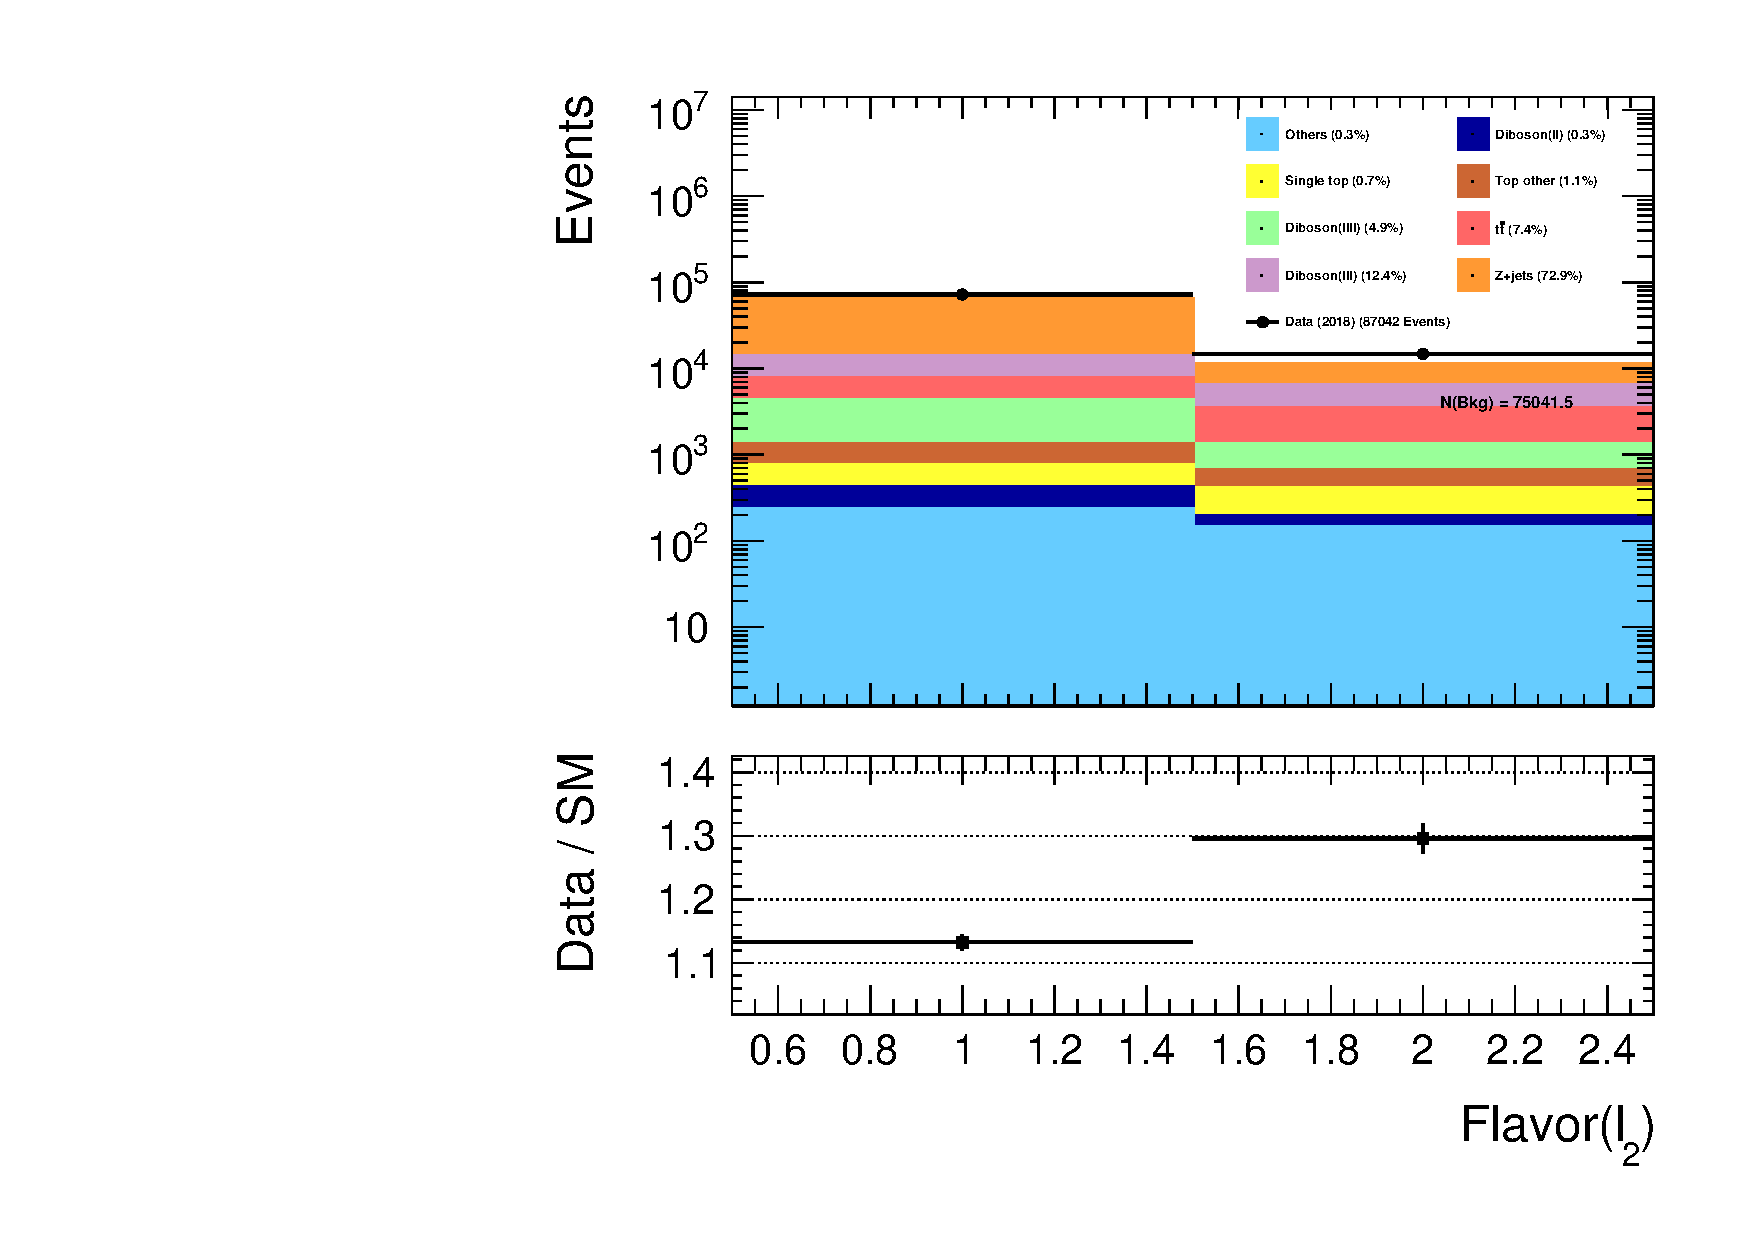
\includegraphics[width=\textwidth]{Figures/FeaturesHistograms/lep2_Flavor.pdf}
        \caption{}
        \label{fig:lep2_Flavor}
    \end{subfigure}
    \hfill
    \begin{subfigure}{.525\textwidth}
        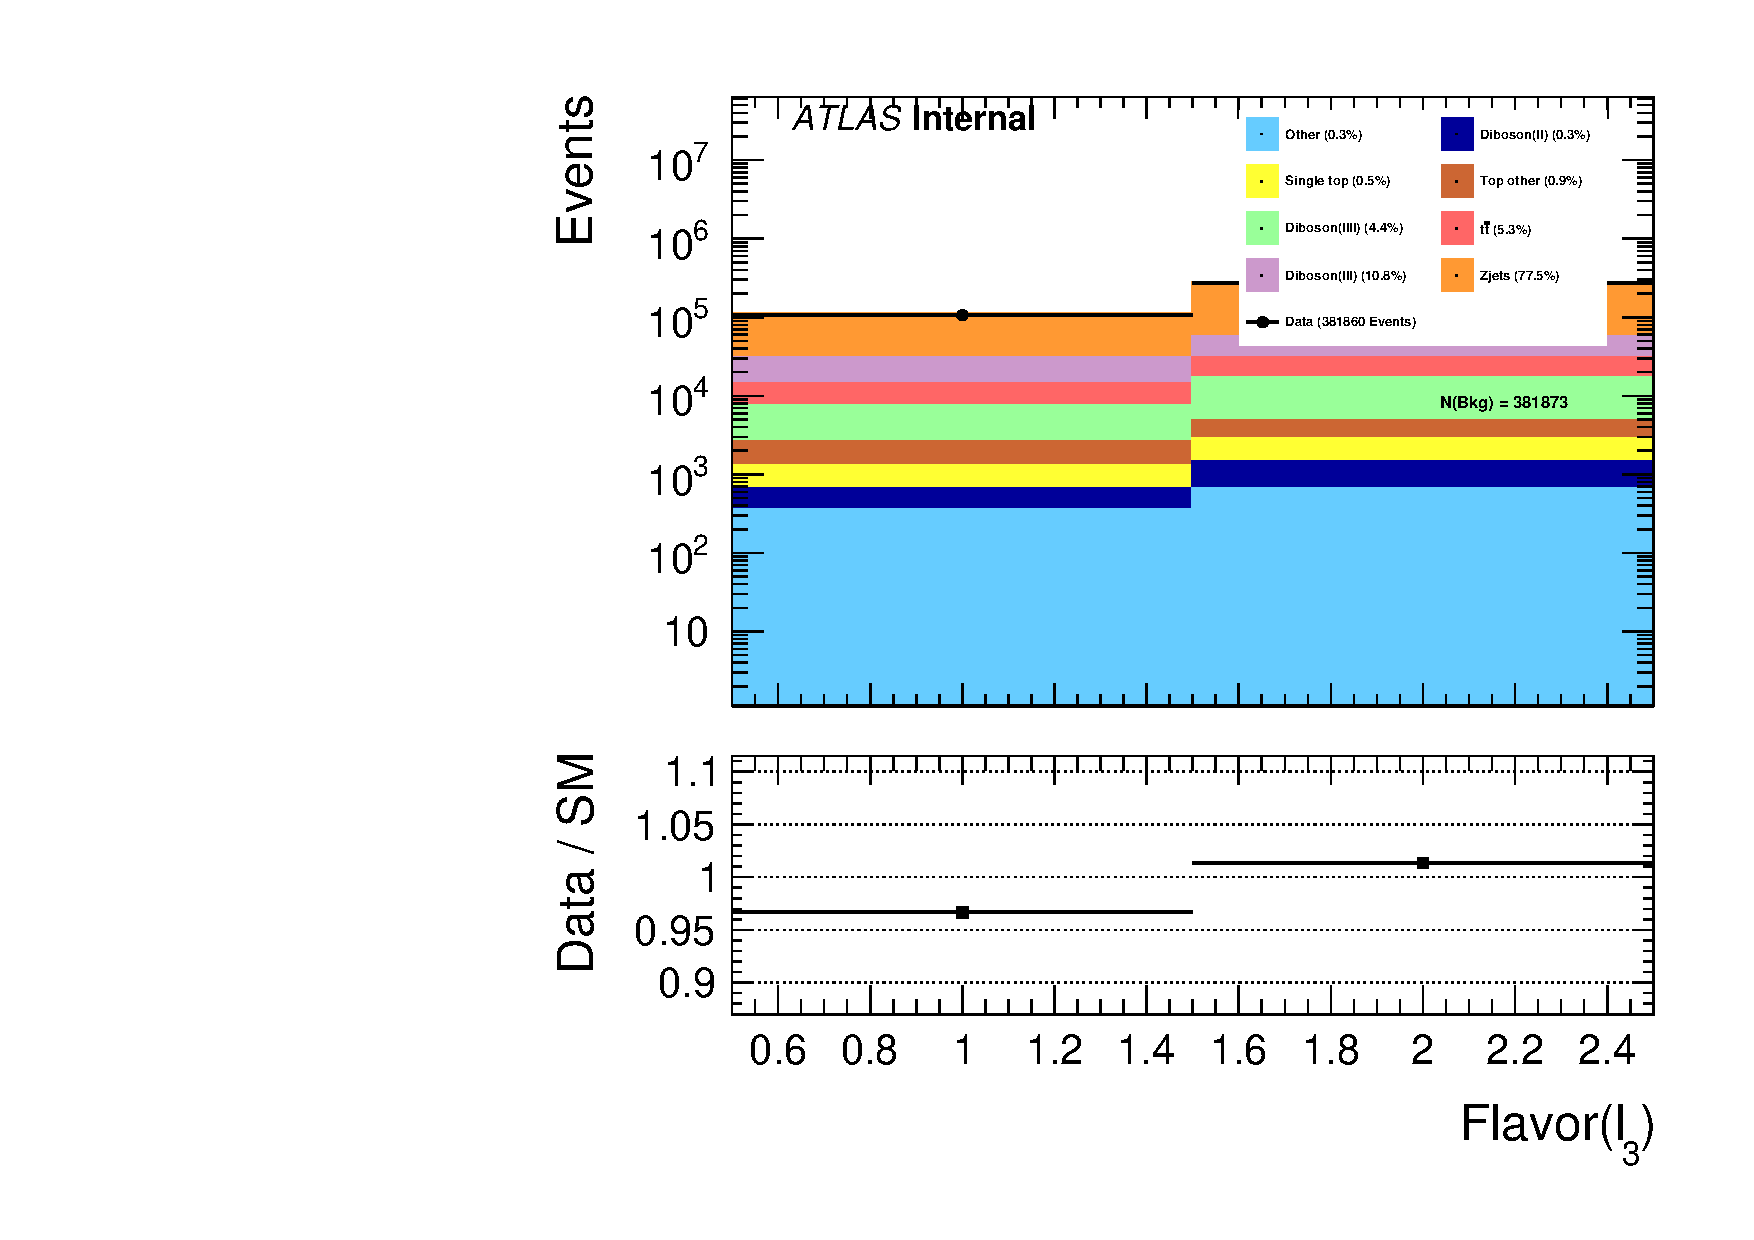
\includegraphics[width=\textwidth]{Figures/FeaturesHistograms/lep3_Flavor.pdf}
        \caption{}
        \label{fig:lep3_Flavor}
    \end{subfigure}
    }
    \caption[\ac{MC} simulated and measured data comparison and event distribution for each channel over the charge for the first,
    second and third lepton. Similarly, the distribution over the flavor for the first, second and third lepton]{\ac{MC} simulated and measured data 
    comparison and event distribution for each channel over the charge for the first \ref{fig:lep1_Charge},
    second \ref{fig:lep2_Charge} and third \ref{fig:lep3_Charge} lepton. Similarly, the distribution over the flavor
    for the first \ref{fig:lep1_Flavor}, second \ref{fig:lep2_Flavor} and third \ref{fig:lep3_Flavor} lepton.}
\end{figure}
\newpage
\begin{figure}[H]
    \makebox[0.95\linewidth][c]{%
    \centering
    \begin{subfigure}{.405\textwidth}
        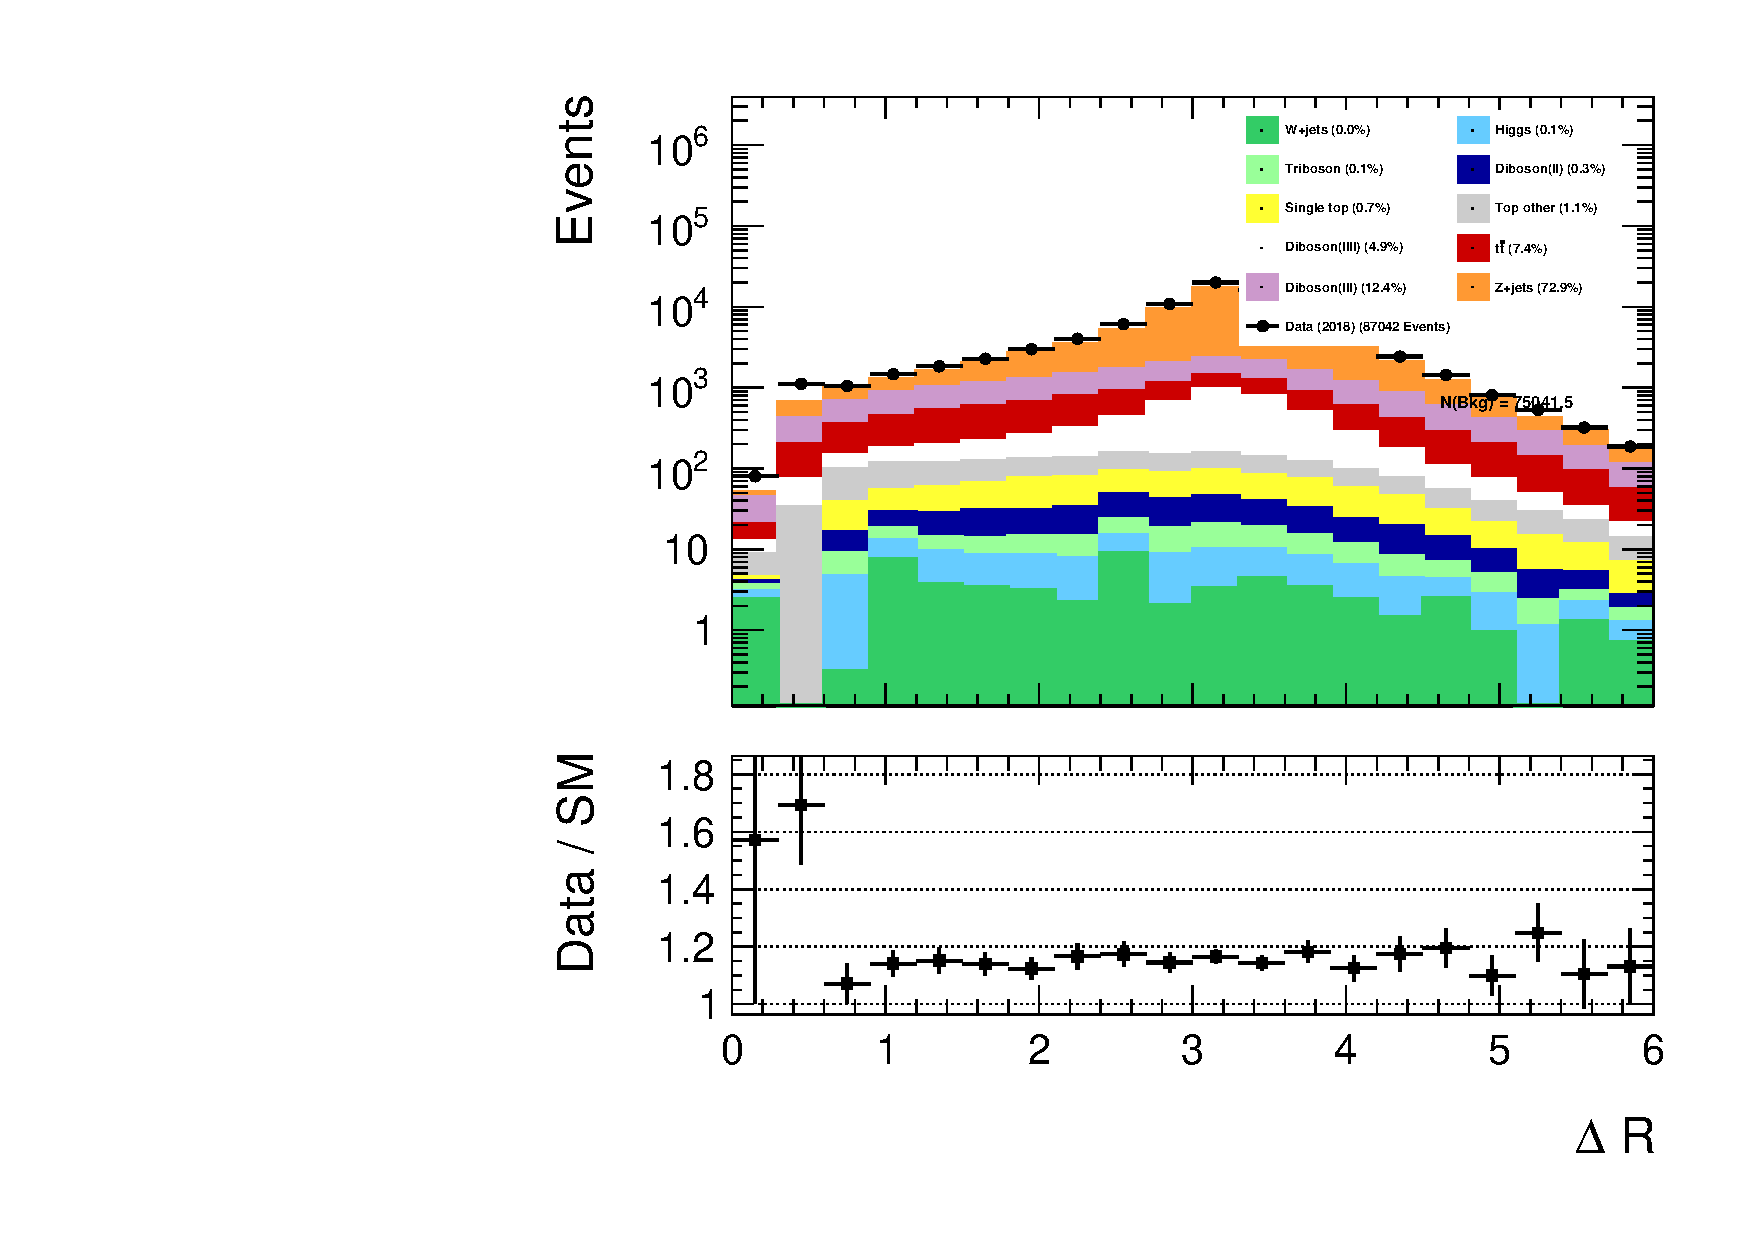
\includegraphics[width=\textwidth]{Figures/FeaturesHistograms/deltaR.pdf}
        \caption{}
        \label{fig:deltaR}
    \end{subfigure}
    \hfill
    \begin{subfigure}{.525\textwidth}
        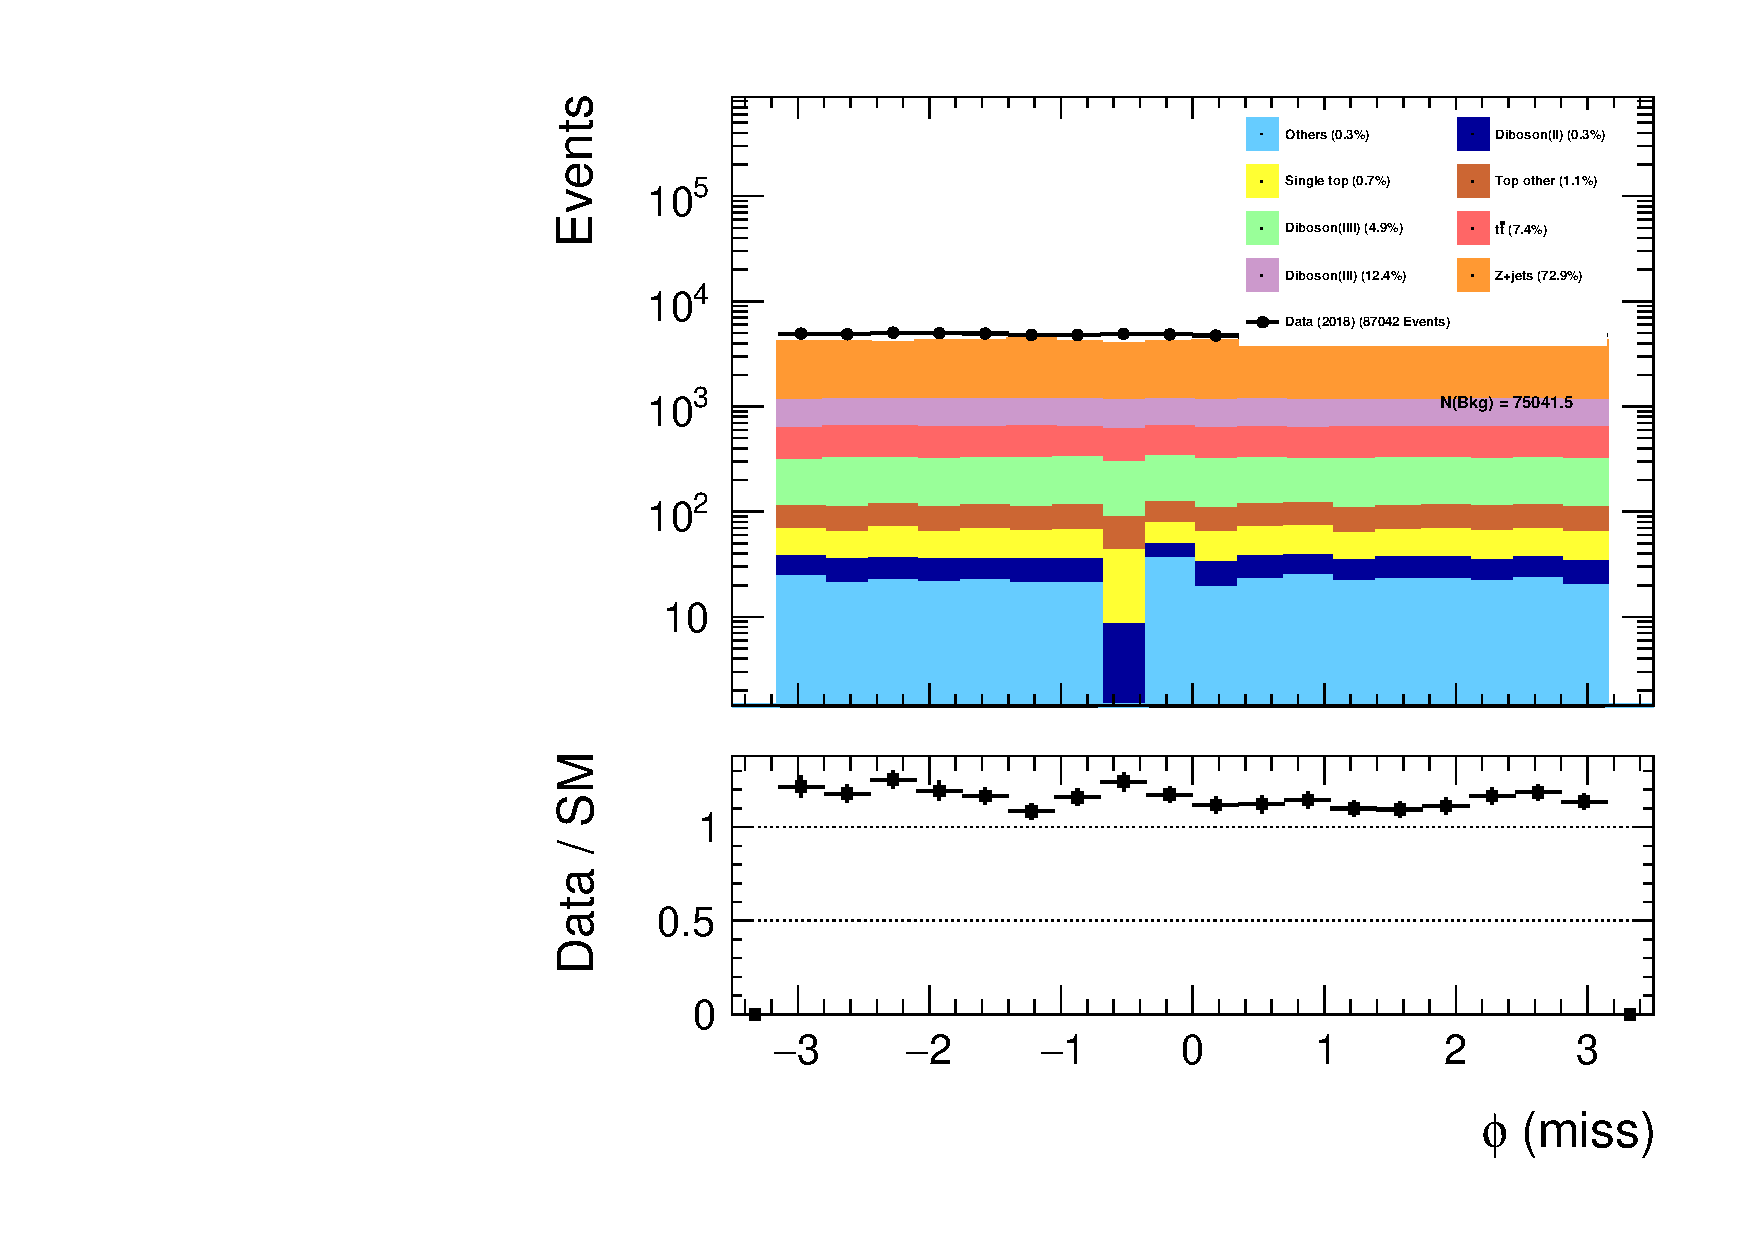
\includegraphics[width=\textwidth]{Figures/FeaturesHistograms/met_Phi.pdf}
        \caption{}
        \label{fig:met_Phi}
    \end{subfigure}
    }
    \makebox[0.95\linewidth][c]{%
    \begin{subfigure}{.405\textwidth}
        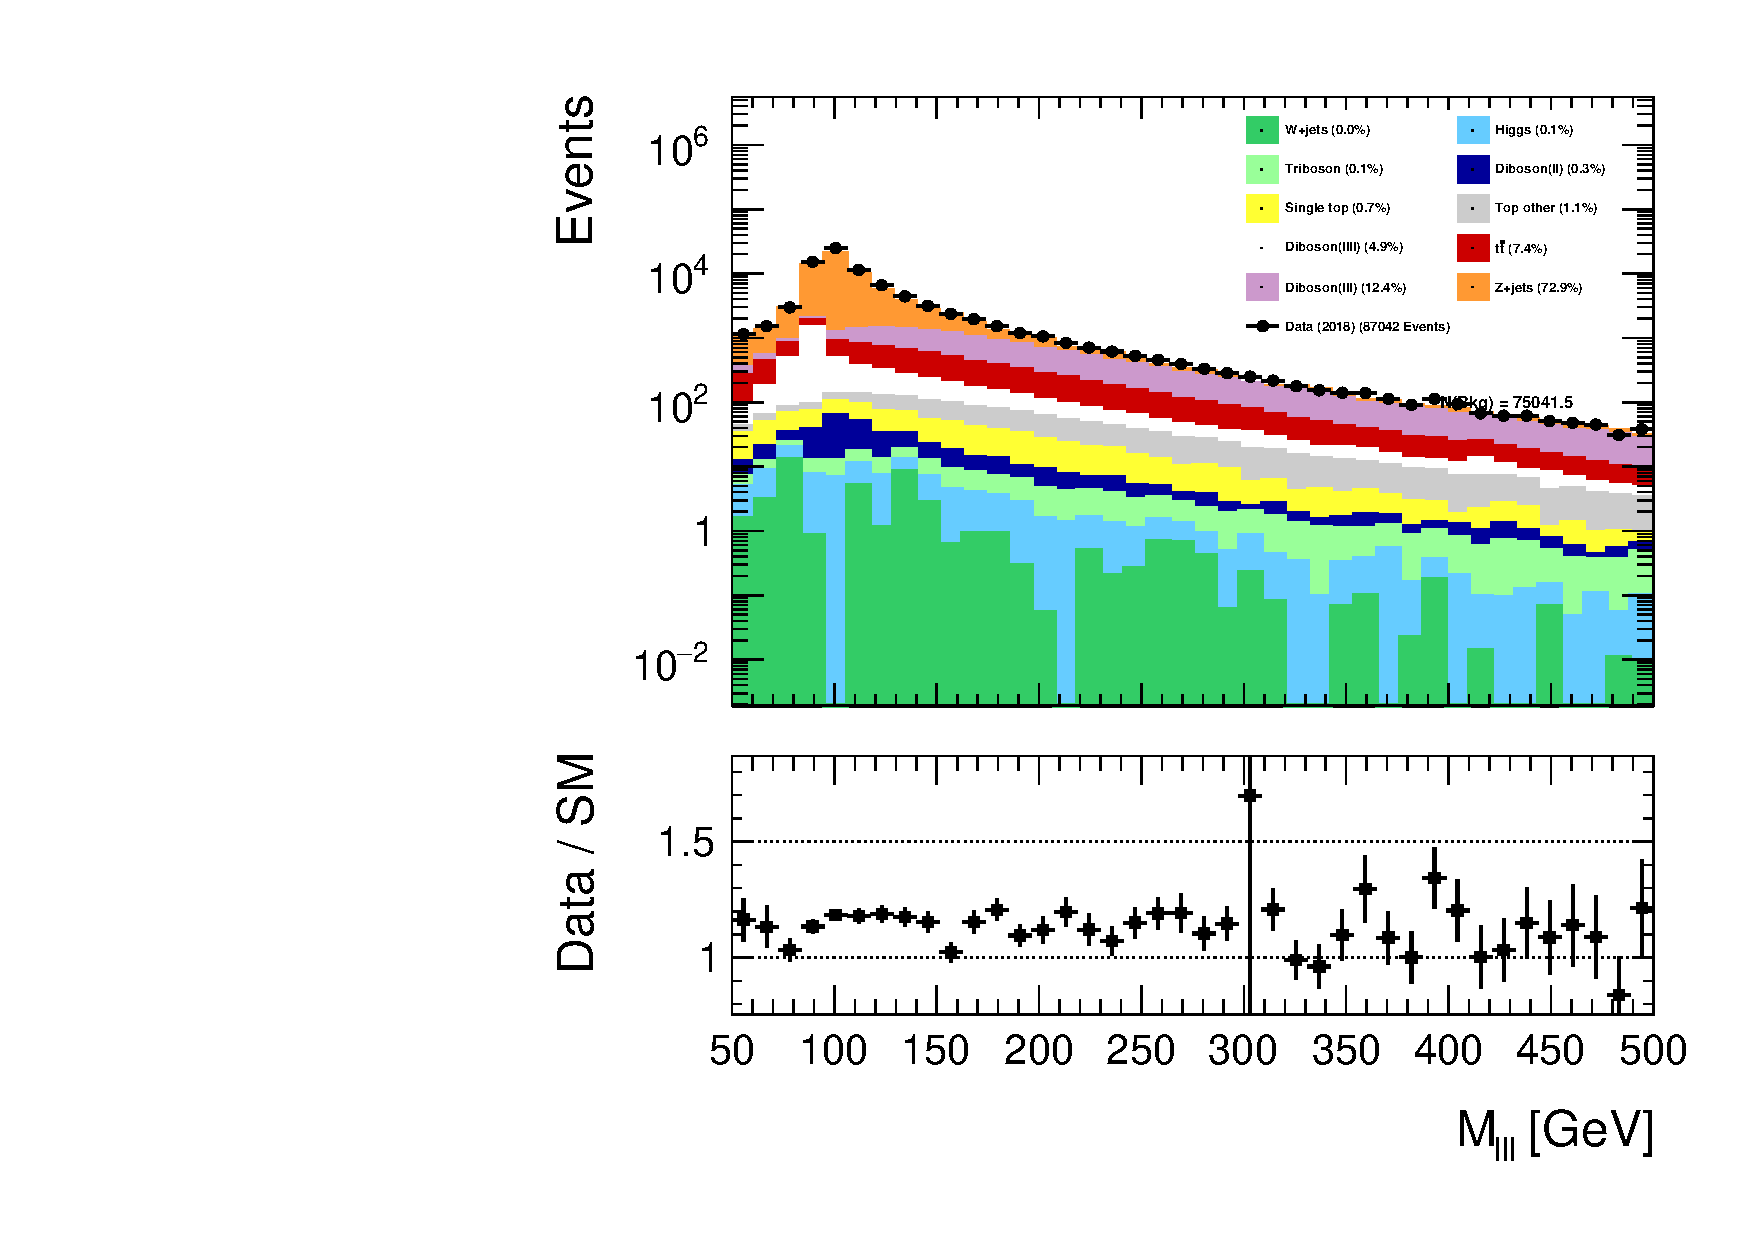
\includegraphics[width=\textwidth]{Figures/FeaturesHistograms/mlll.pdf}
        \caption{}
        \label{fig:mlll}
    \end{subfigure}
    \hfill
    \begin{subfigure}{.525\textwidth}
        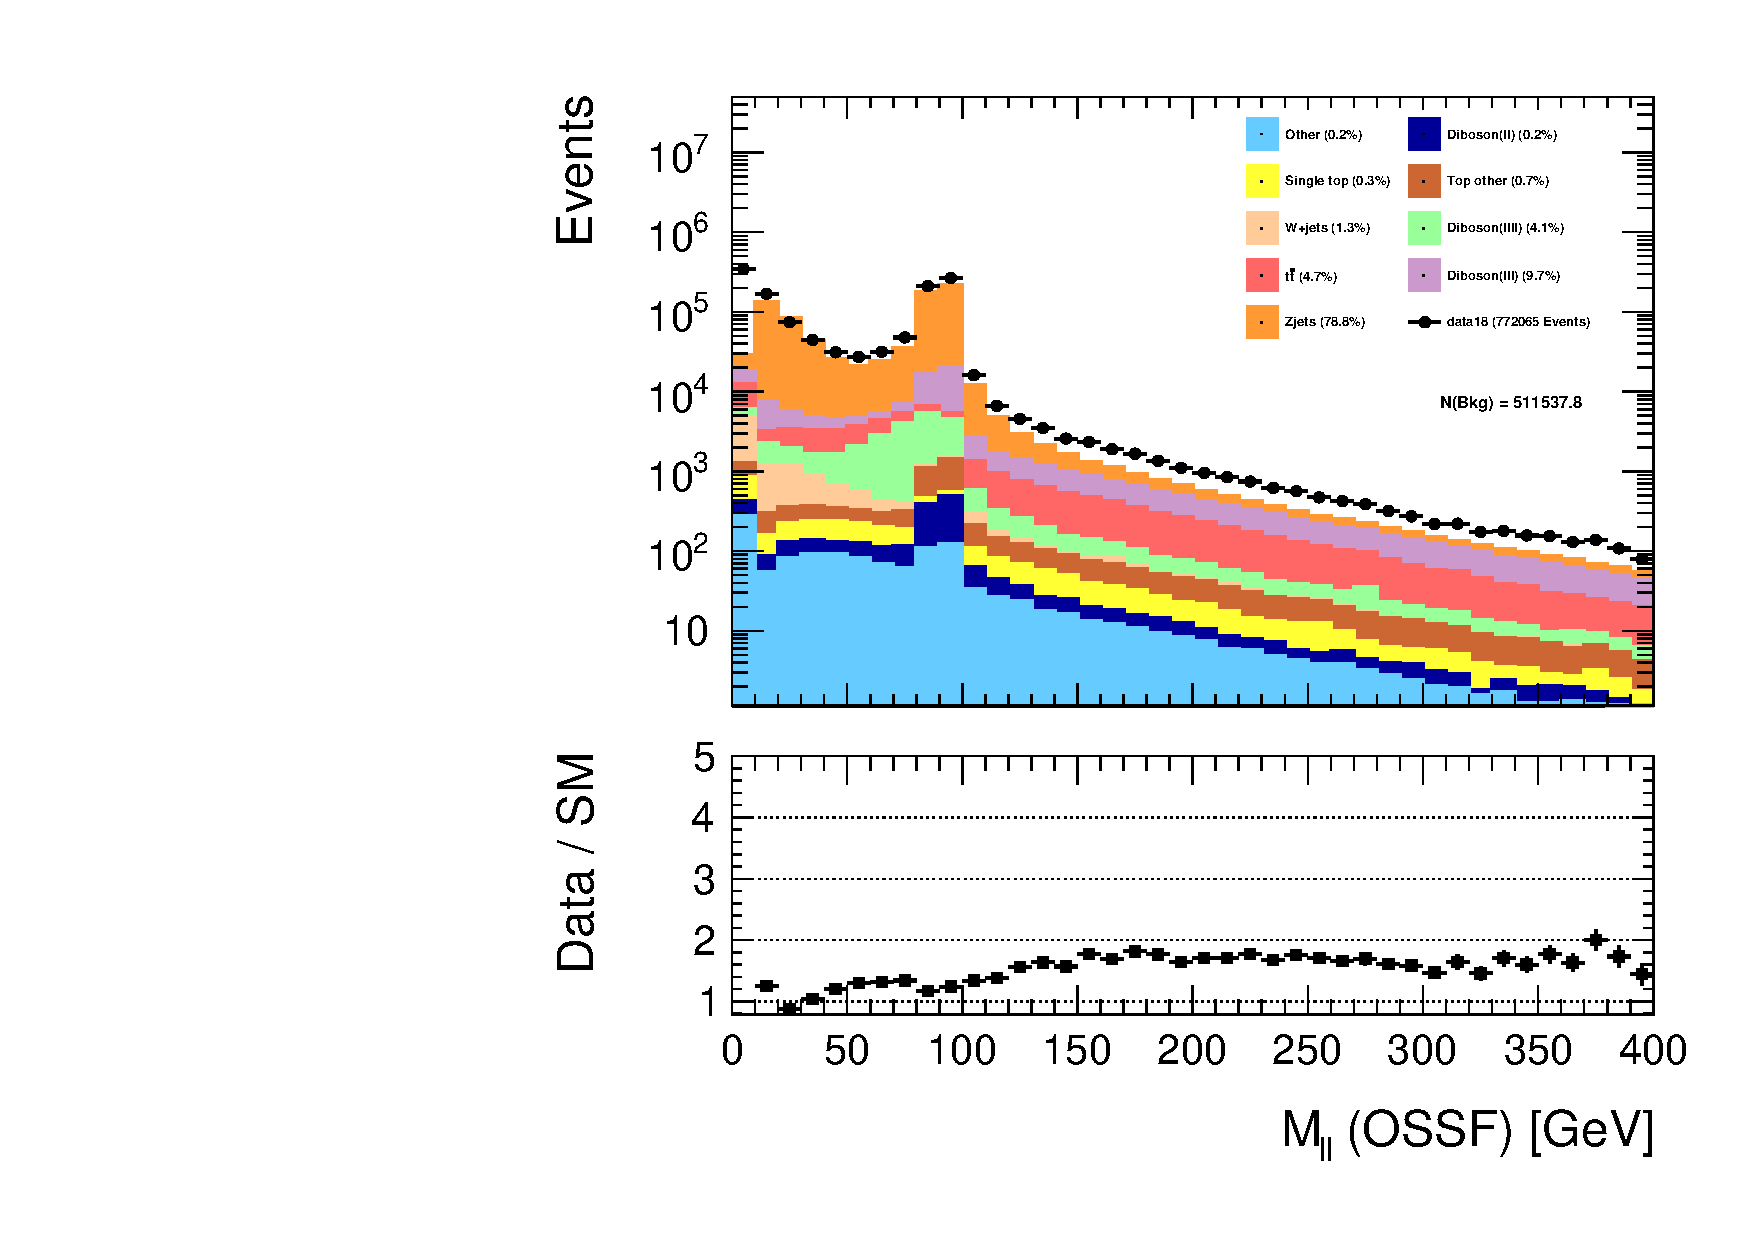
\includegraphics[width=\textwidth]{Figures/FeaturesHistograms/mll_OSSF.pdf}
        \caption{}
        \label{fig:mll_OSSF}
    \end{subfigure}
    }
    \makebox[0.95\linewidth][c]{%
    \begin{subfigure}{.405\textwidth}
        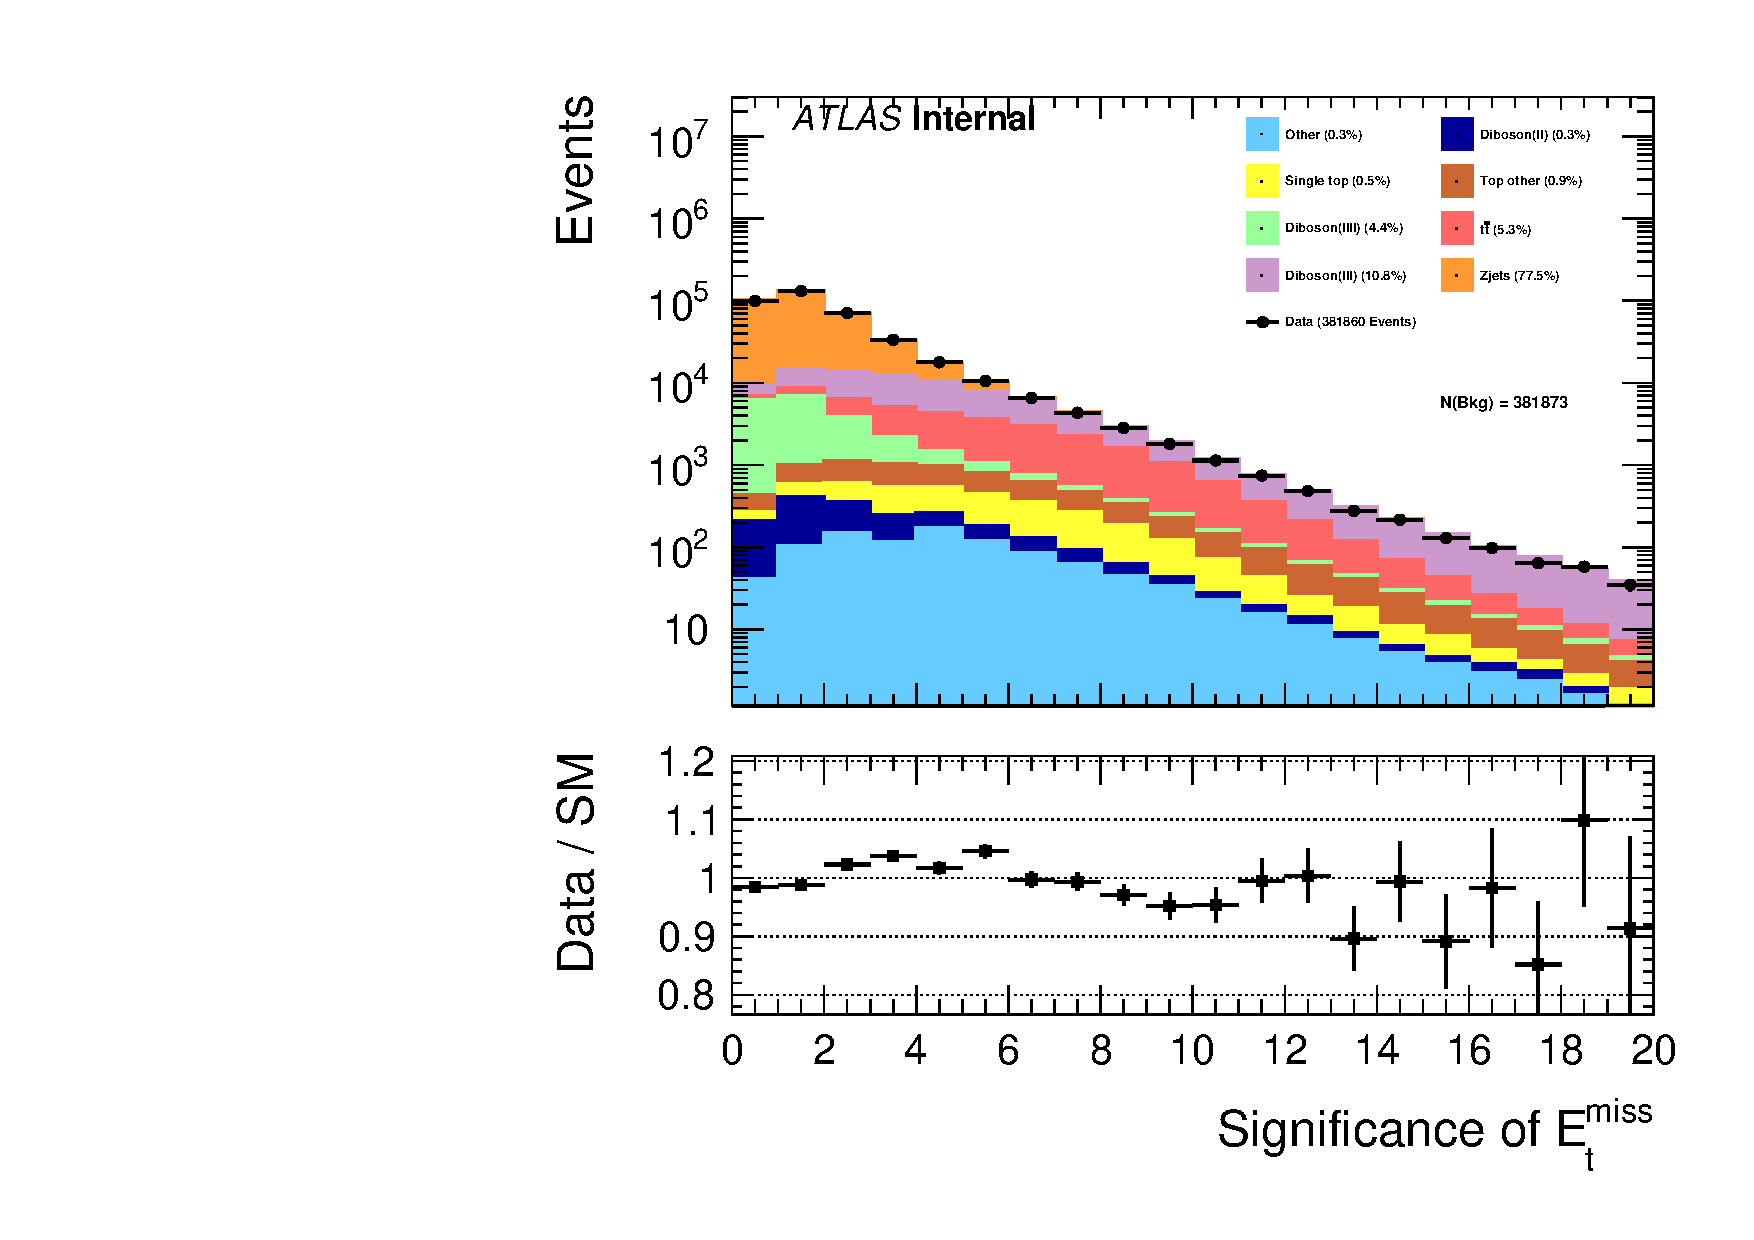
\includegraphics[width=\textwidth]{Figures/FeaturesHistograms/met_Sign.pdf}
        \caption{}
        \label{fig:met_Sign}
    \end{subfigure}
    \hfill
    \begin{subfigure}{.525\textwidth}
        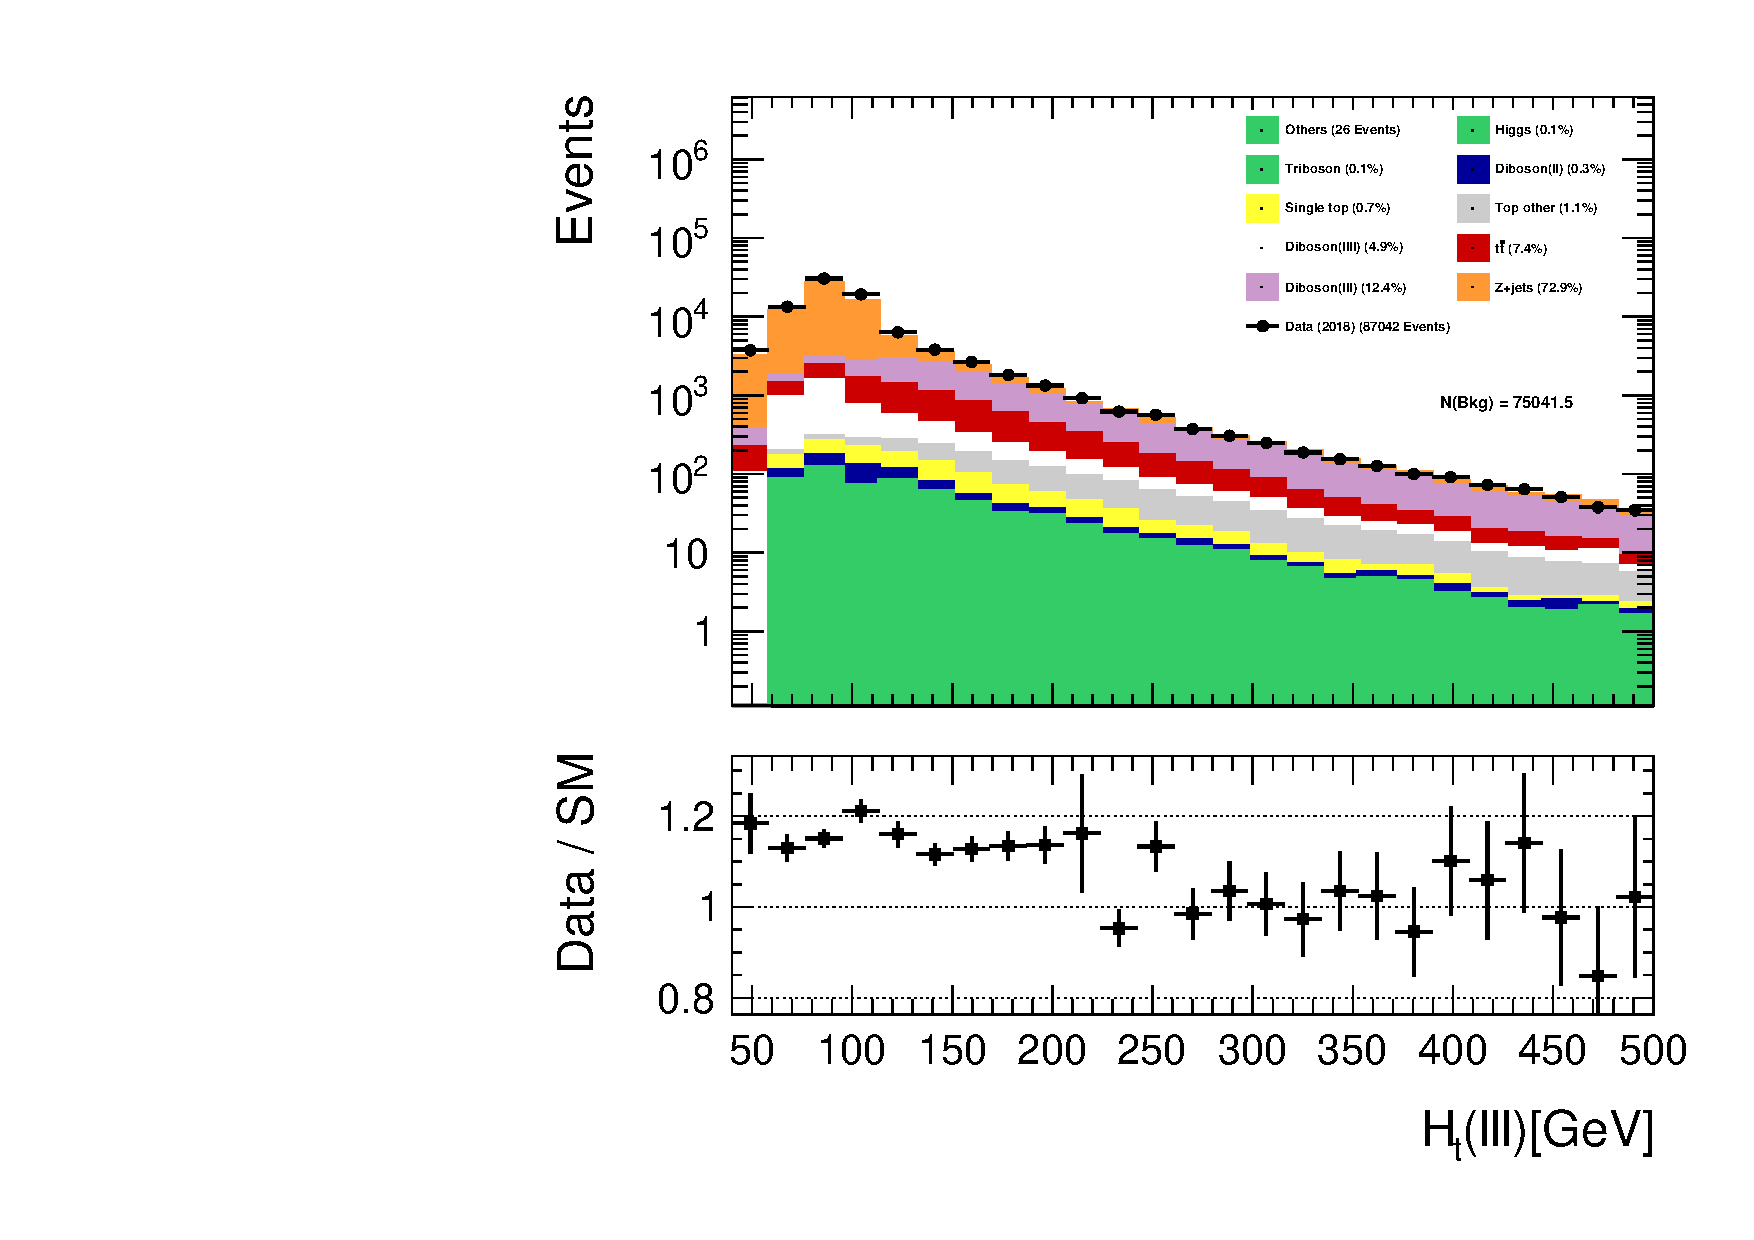
\includegraphics[width=\textwidth]{Figures/FeaturesHistograms/Ht_lll.pdf}
        \caption{}
        \label{fig:Ht_lll}
    \end{subfigure}
    }
    \caption[\ac{MC} simulated and measured data comparison and event distribution for each channel over $\Delta R$ \ref{fig:deltaR}
    and the azimuthal angle of the missing energy. The distribution of the invariant mass of the three leptons and the OSSF pair. 
    The distribution over the significance of the missing transverse energy and the sum of $P_t$.]{\ac{MC} simulated and measured data 
    comparison and event distribution for each channel over $\Delta R$ \ref{fig:deltaR} and the azimuthal
    angel \ref{fig:met_Phi} of the missing energy. The distribution of the invariant mass of the
    three leptons \ref{fig:mlll} and the OSSF pair \ref{fig:mll_OSSF}. The distribution over the significance
    of the missing transverse energy \ref{fig:met_Sign} and the sum of $P_t$ \ref{fig:Ht_lll}.}
\end{figure}
\newpage
\begin{figure}[H]
    \makebox[0.95\linewidth][c]{%
    \centering
    \begin{subfigure}{.405\textwidth}
        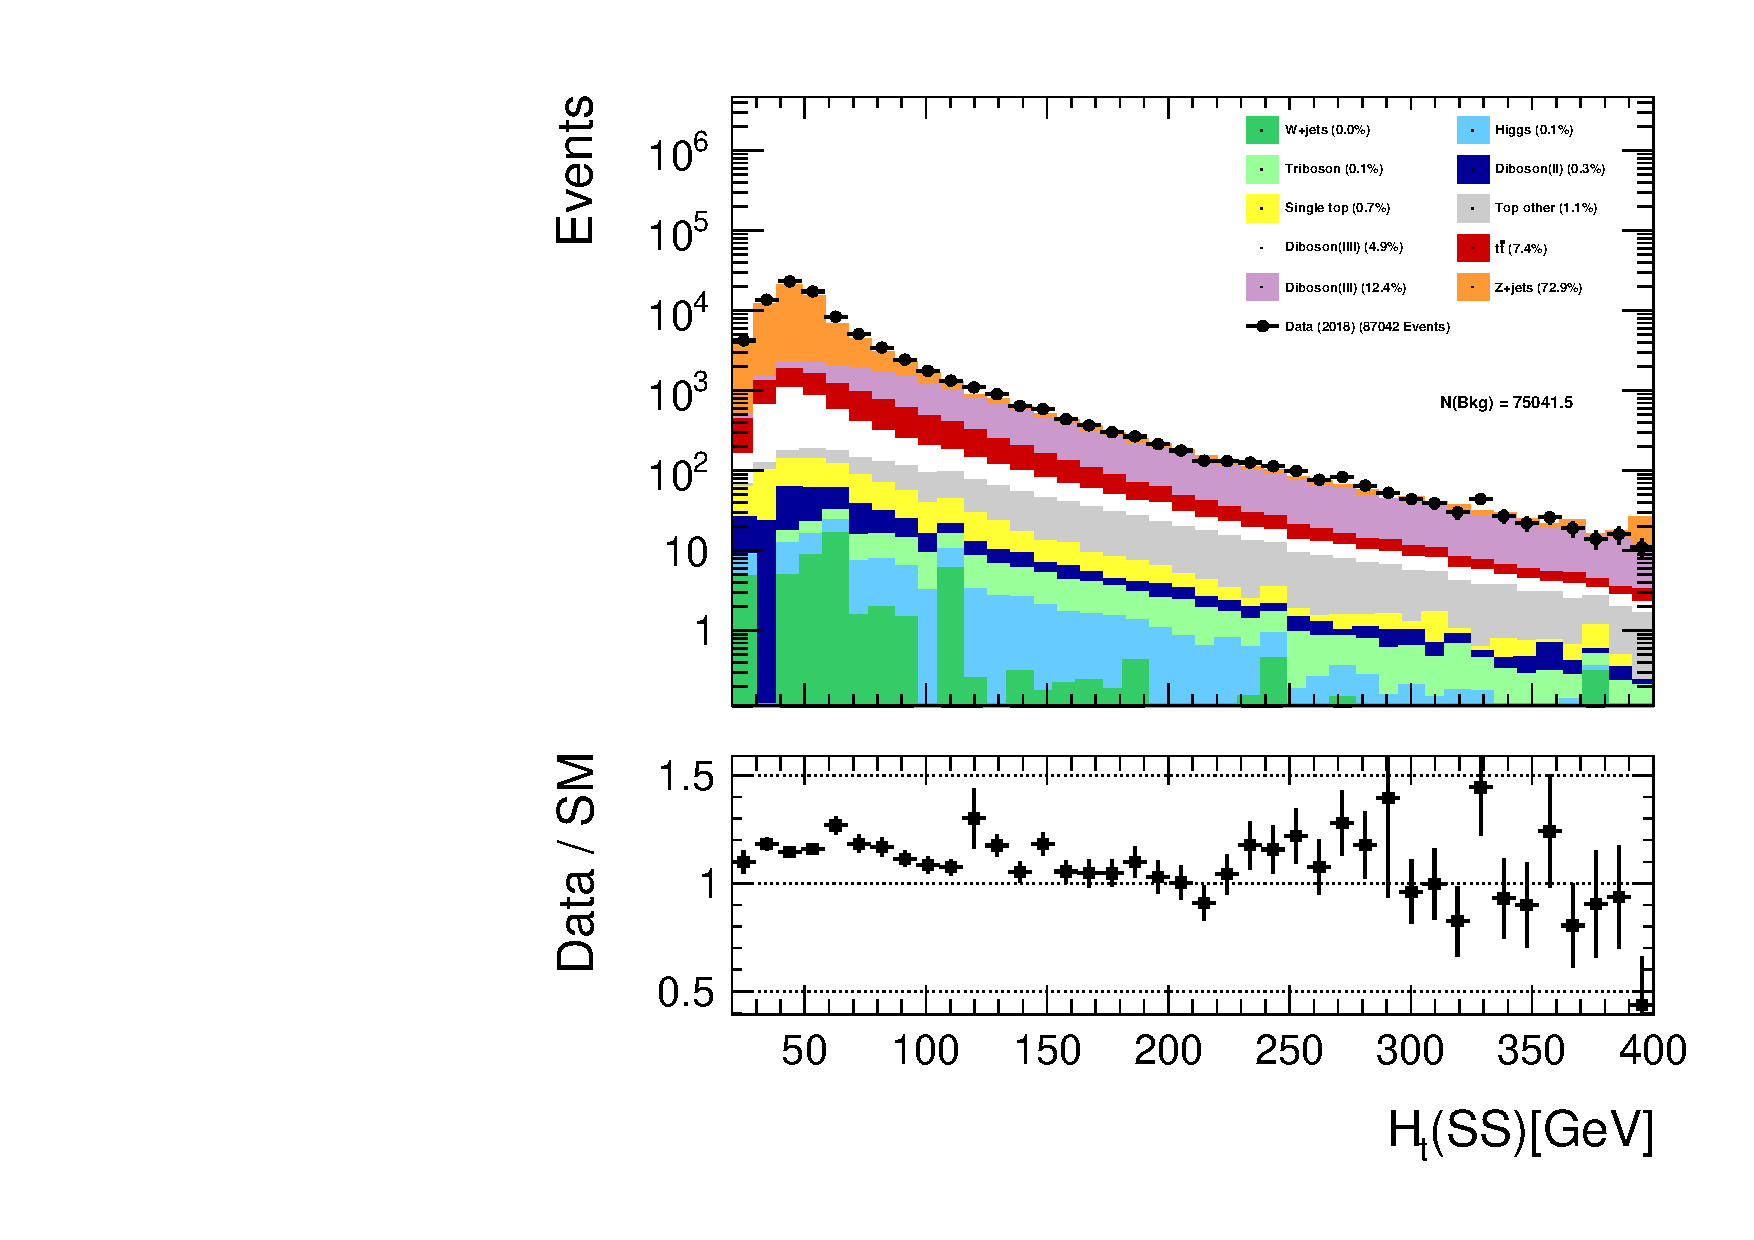
\includegraphics[width=\textwidth]{Figures/FeaturesHistograms/Ht_SS.pdf}
        \caption{}
        \label{fig:Ht_SS}
    \end{subfigure}
    \hfill
    \begin{subfigure}{.525\textwidth}
        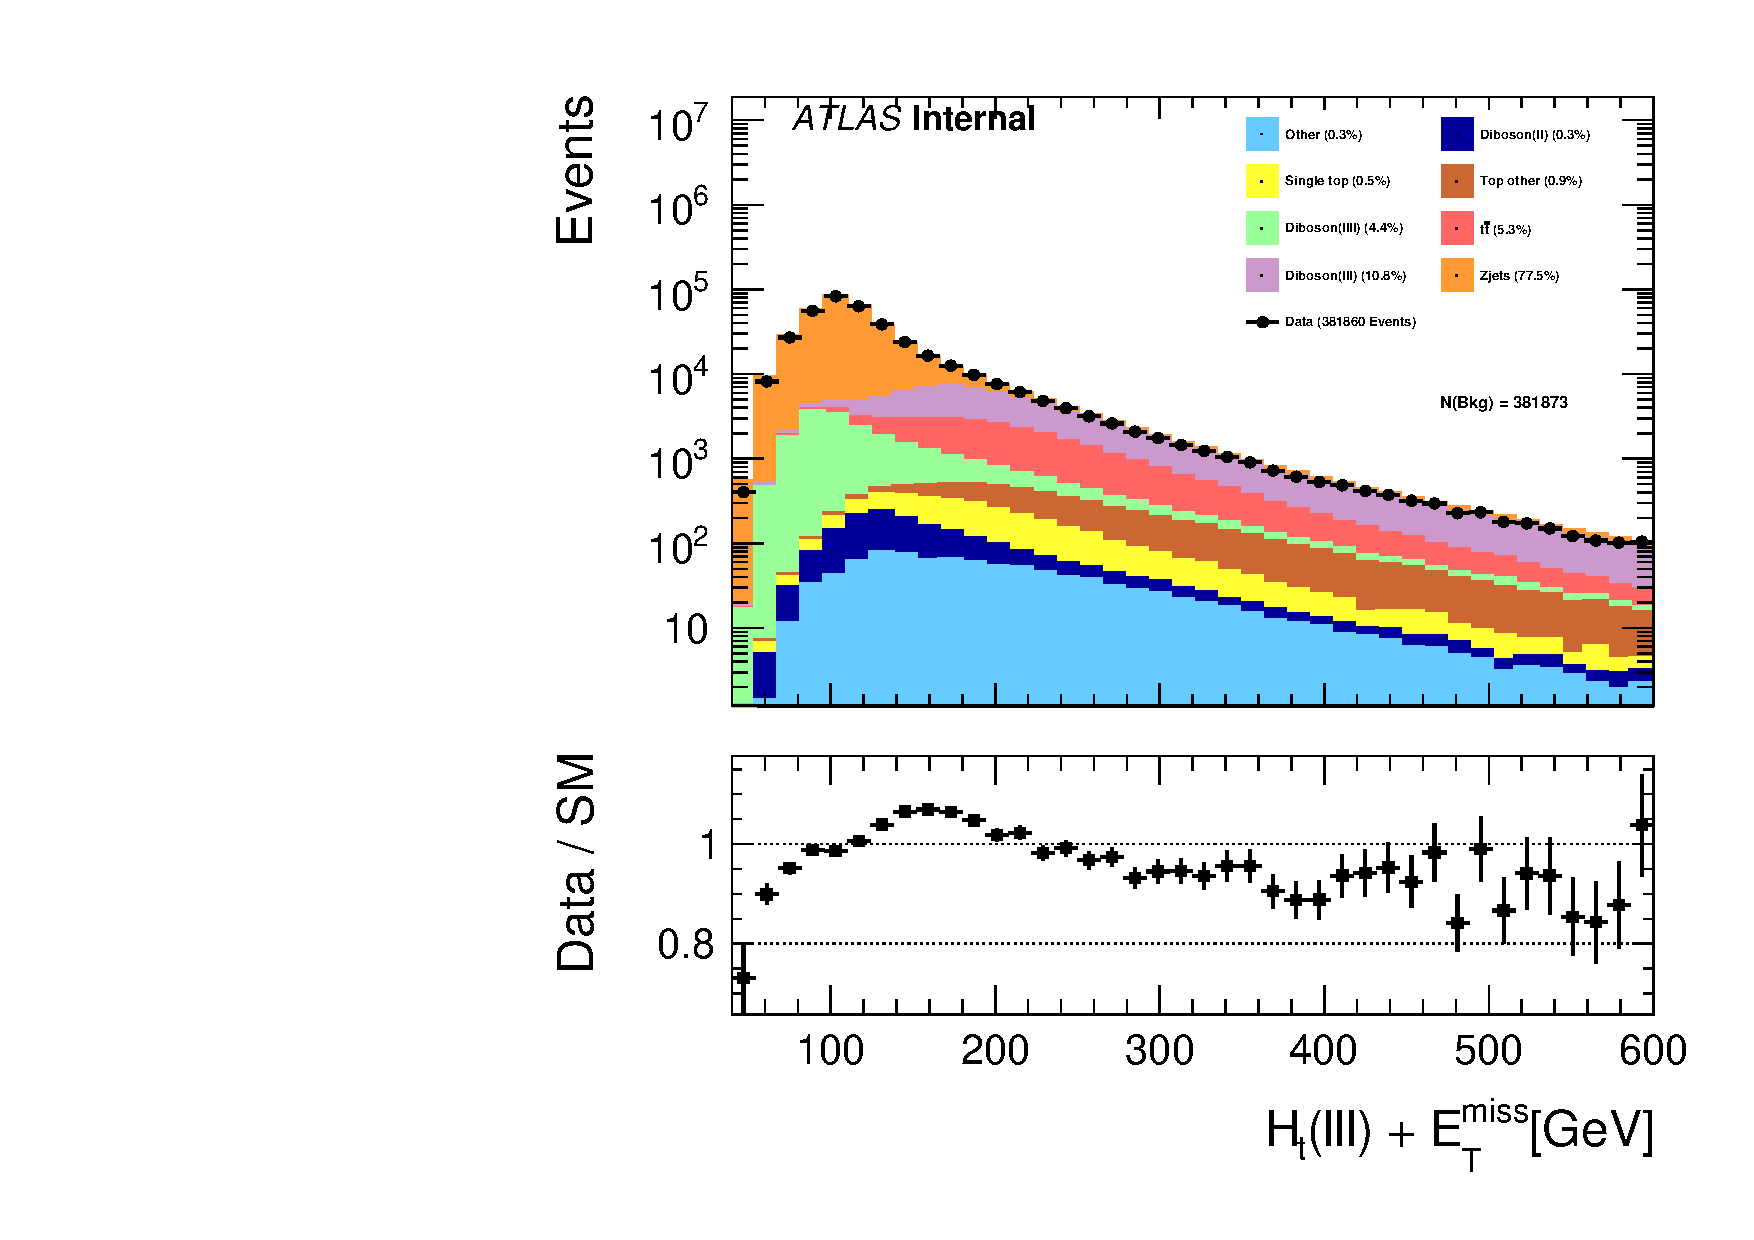
\includegraphics[width=\textwidth]{Figures/FeaturesHistograms/Ht_met_Et.pdf}
        \caption{}
        \label{fig:Ht_met_Et}
    \end{subfigure}
    }
    \makebox[0.95\linewidth][c]{%
    \begin{subfigure}{.405\textwidth}
        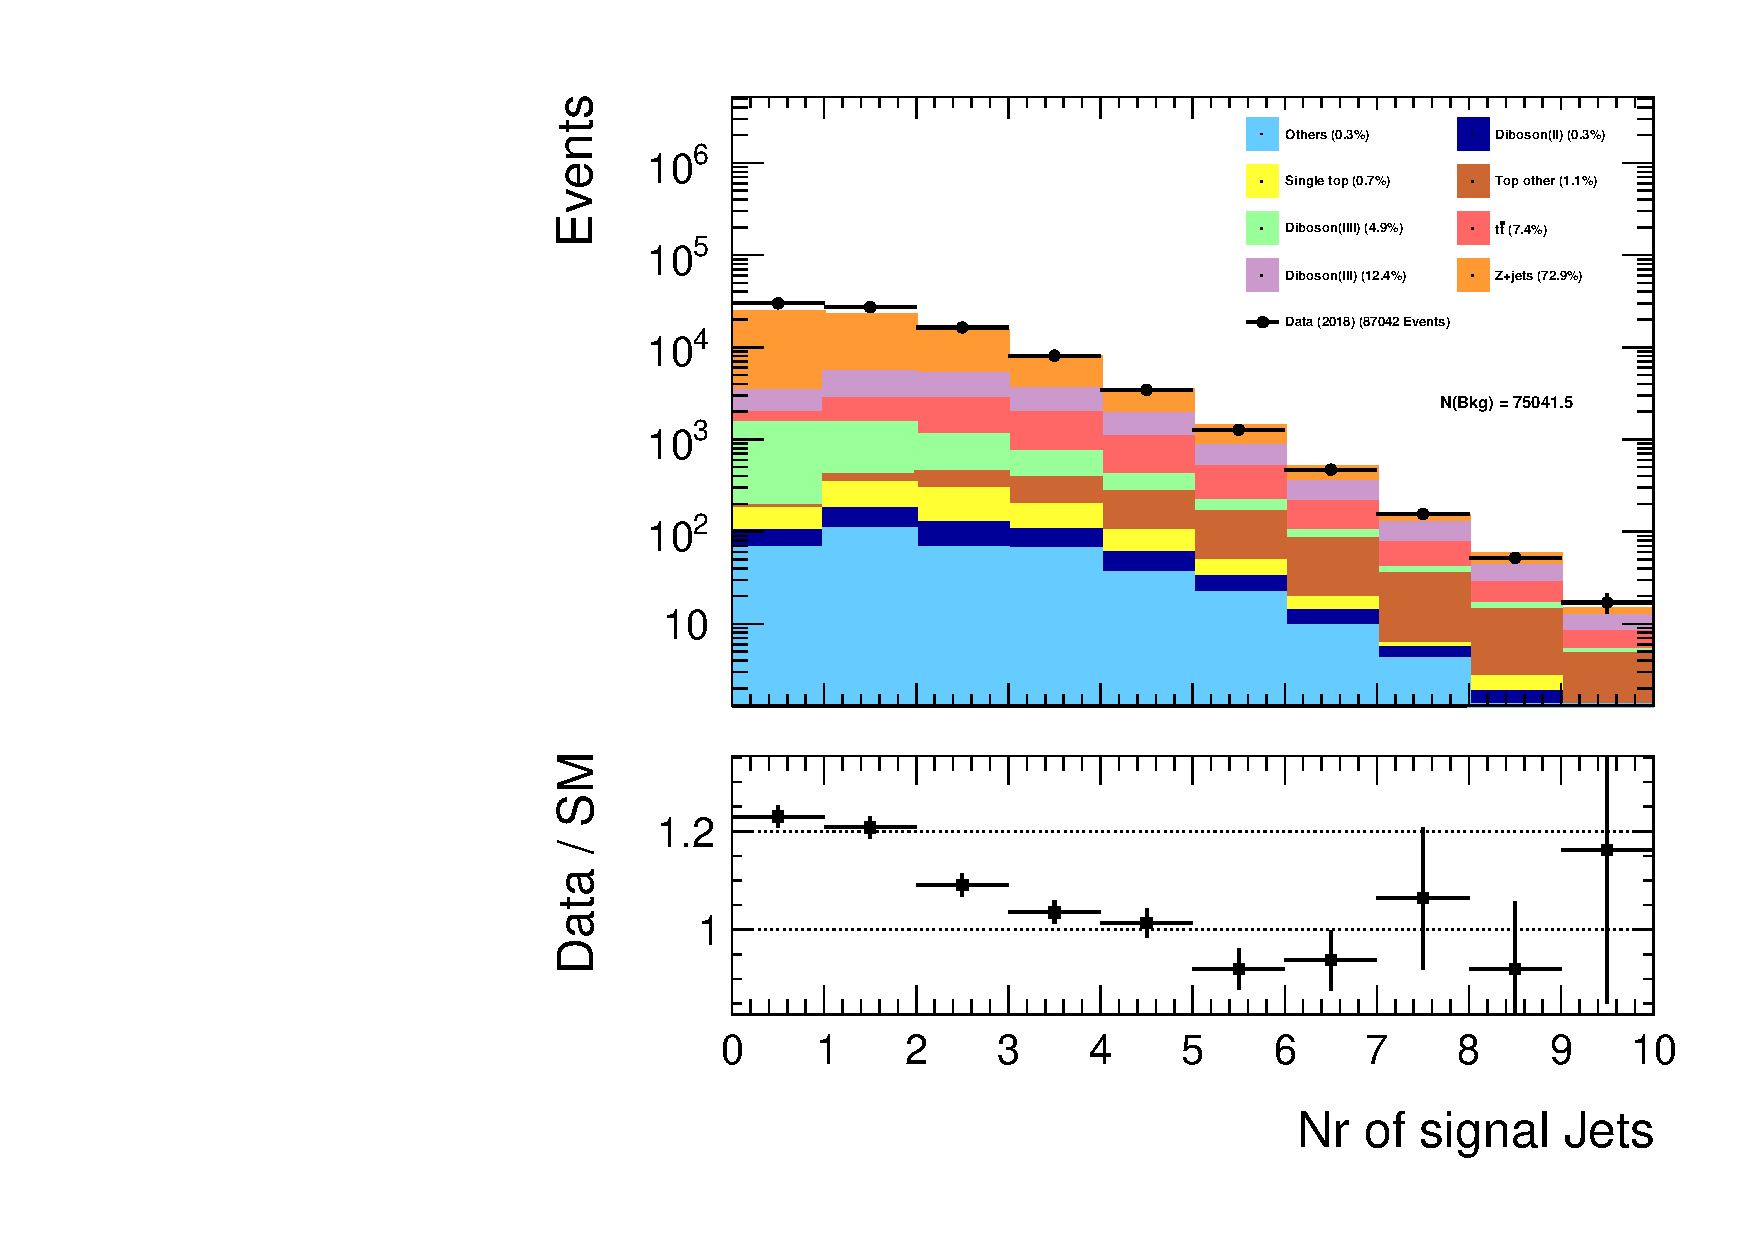
\includegraphics[width=\textwidth]{Figures/FeaturesHistograms/njet_SG.pdf}
        \caption{}
        \label{fig:njet_SG}
    \end{subfigure}
    \hfill
    \begin{subfigure}{.525\textwidth}
        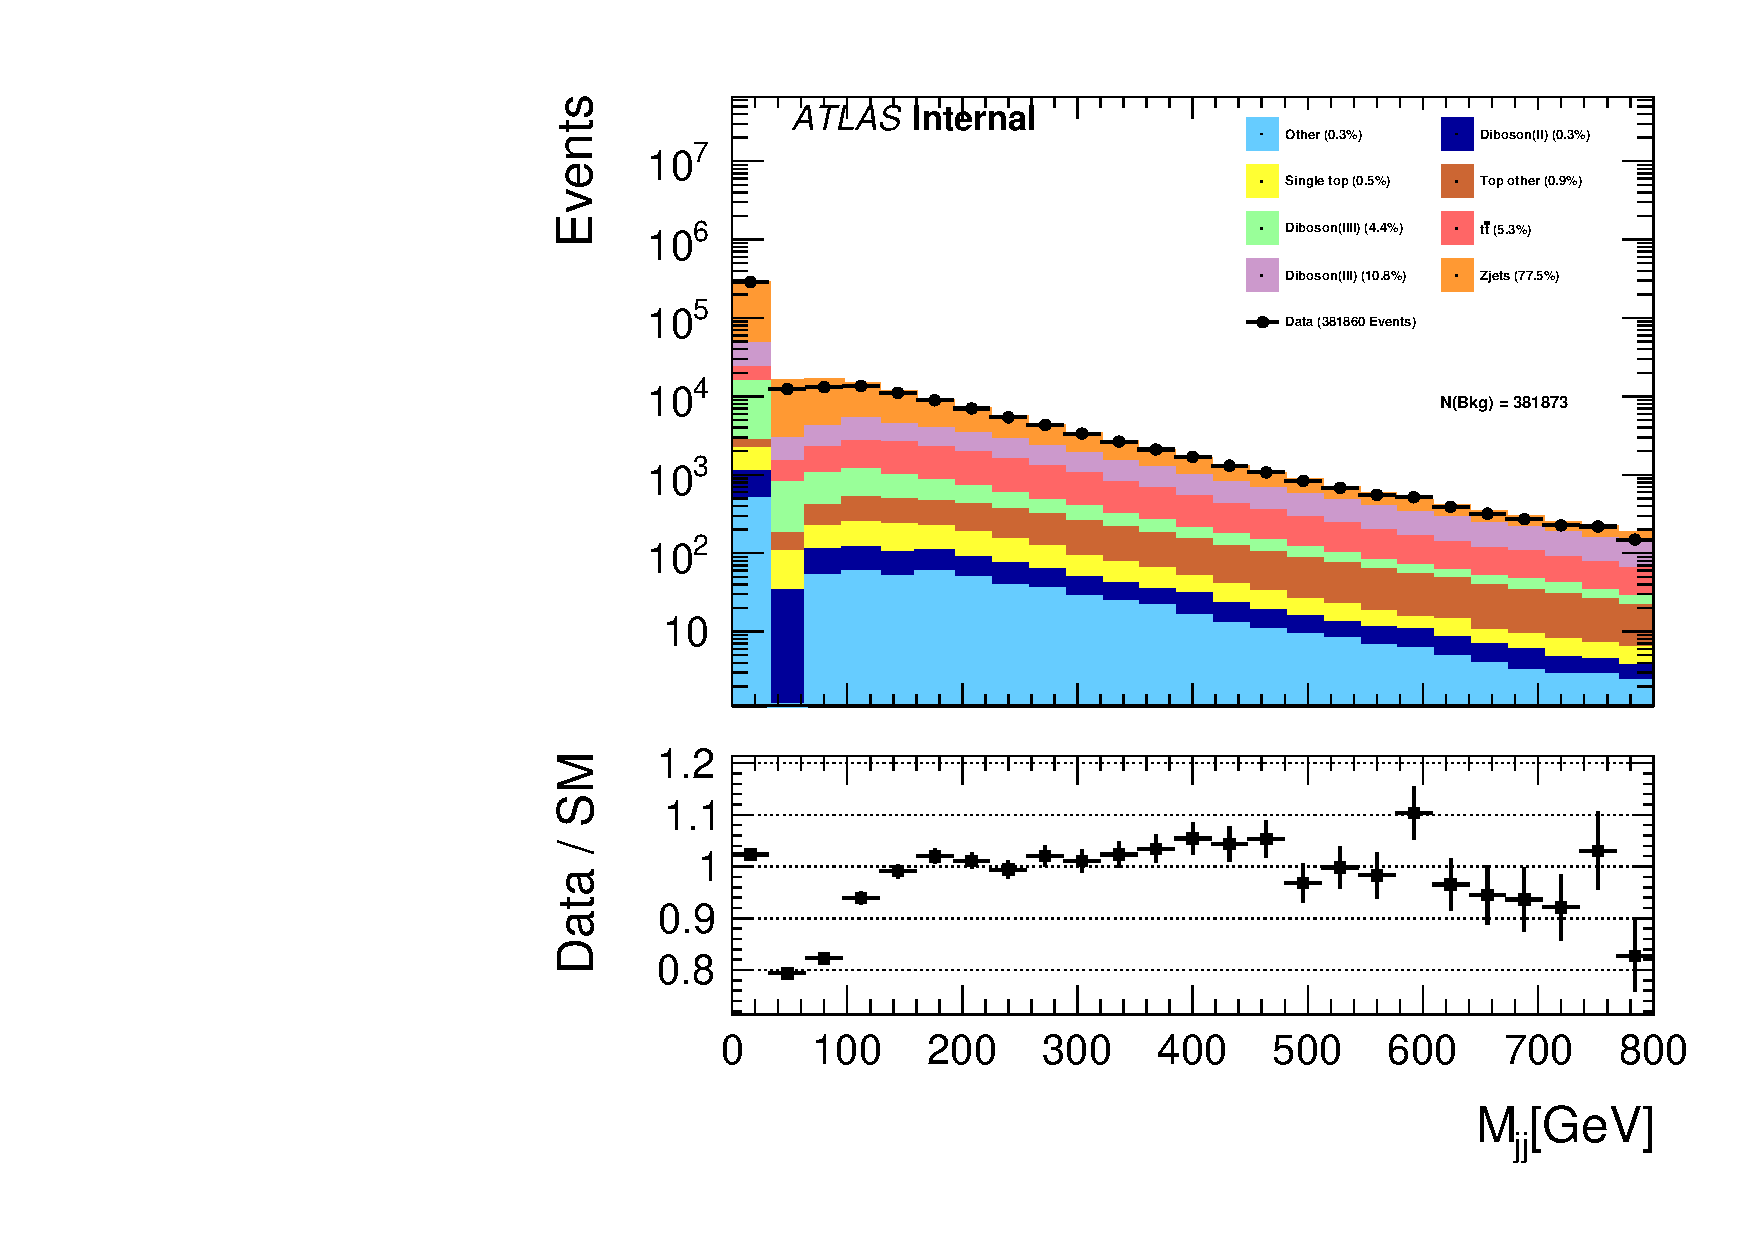
\includegraphics[width=\textwidth]{Figures/FeaturesHistograms/M_jj.pdf}
        \caption{}
        \label{fig:M_jj}
    \end{subfigure}
    }
    \makebox[0.95\linewidth][c]{%
    \centering
    \begin{subfigure}{.405\textwidth}
        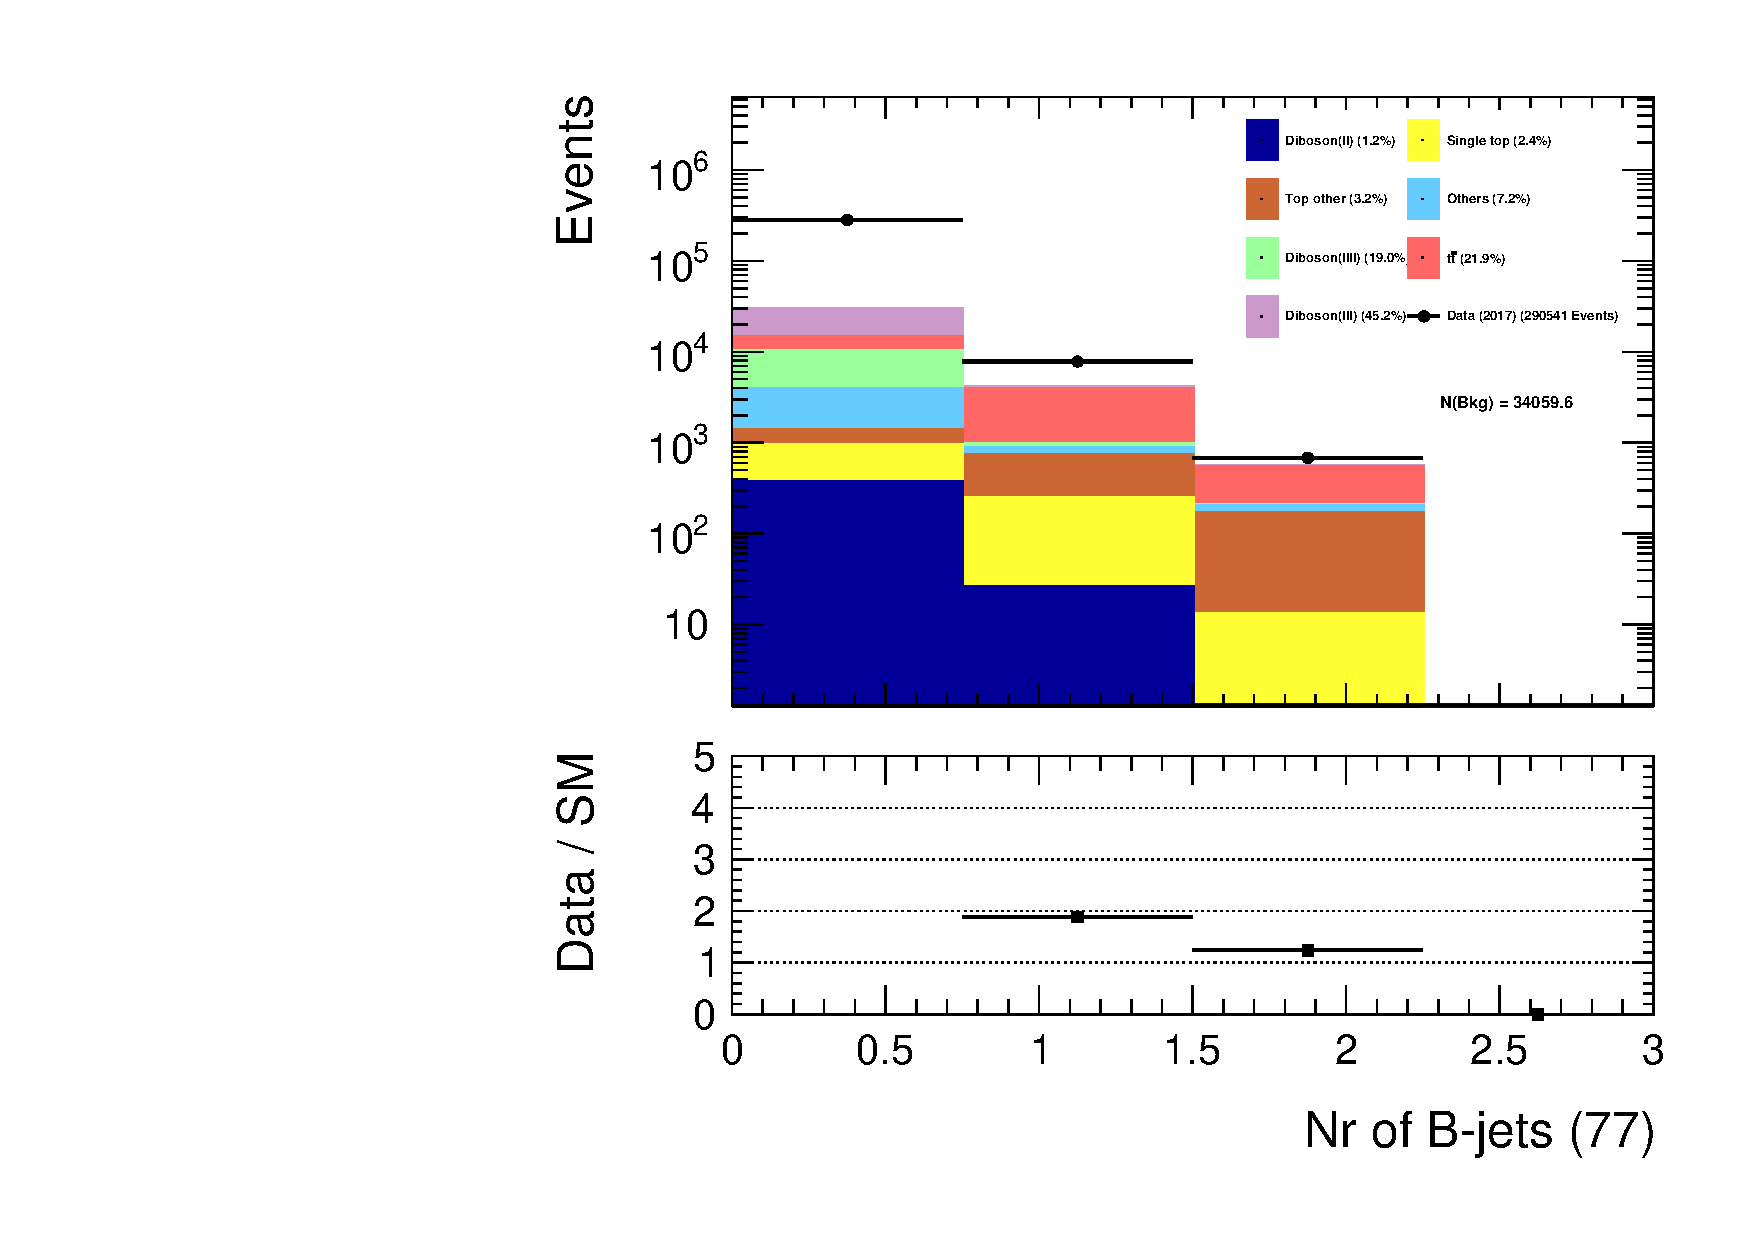
\includegraphics[width=\textwidth]{Figures/FeaturesHistograms/nbjet77.pdf}
        \caption{}
        \label{fig:nbjet77}
    \end{subfigure}
    \hfill
    \begin{subfigure}{.525\textwidth}
        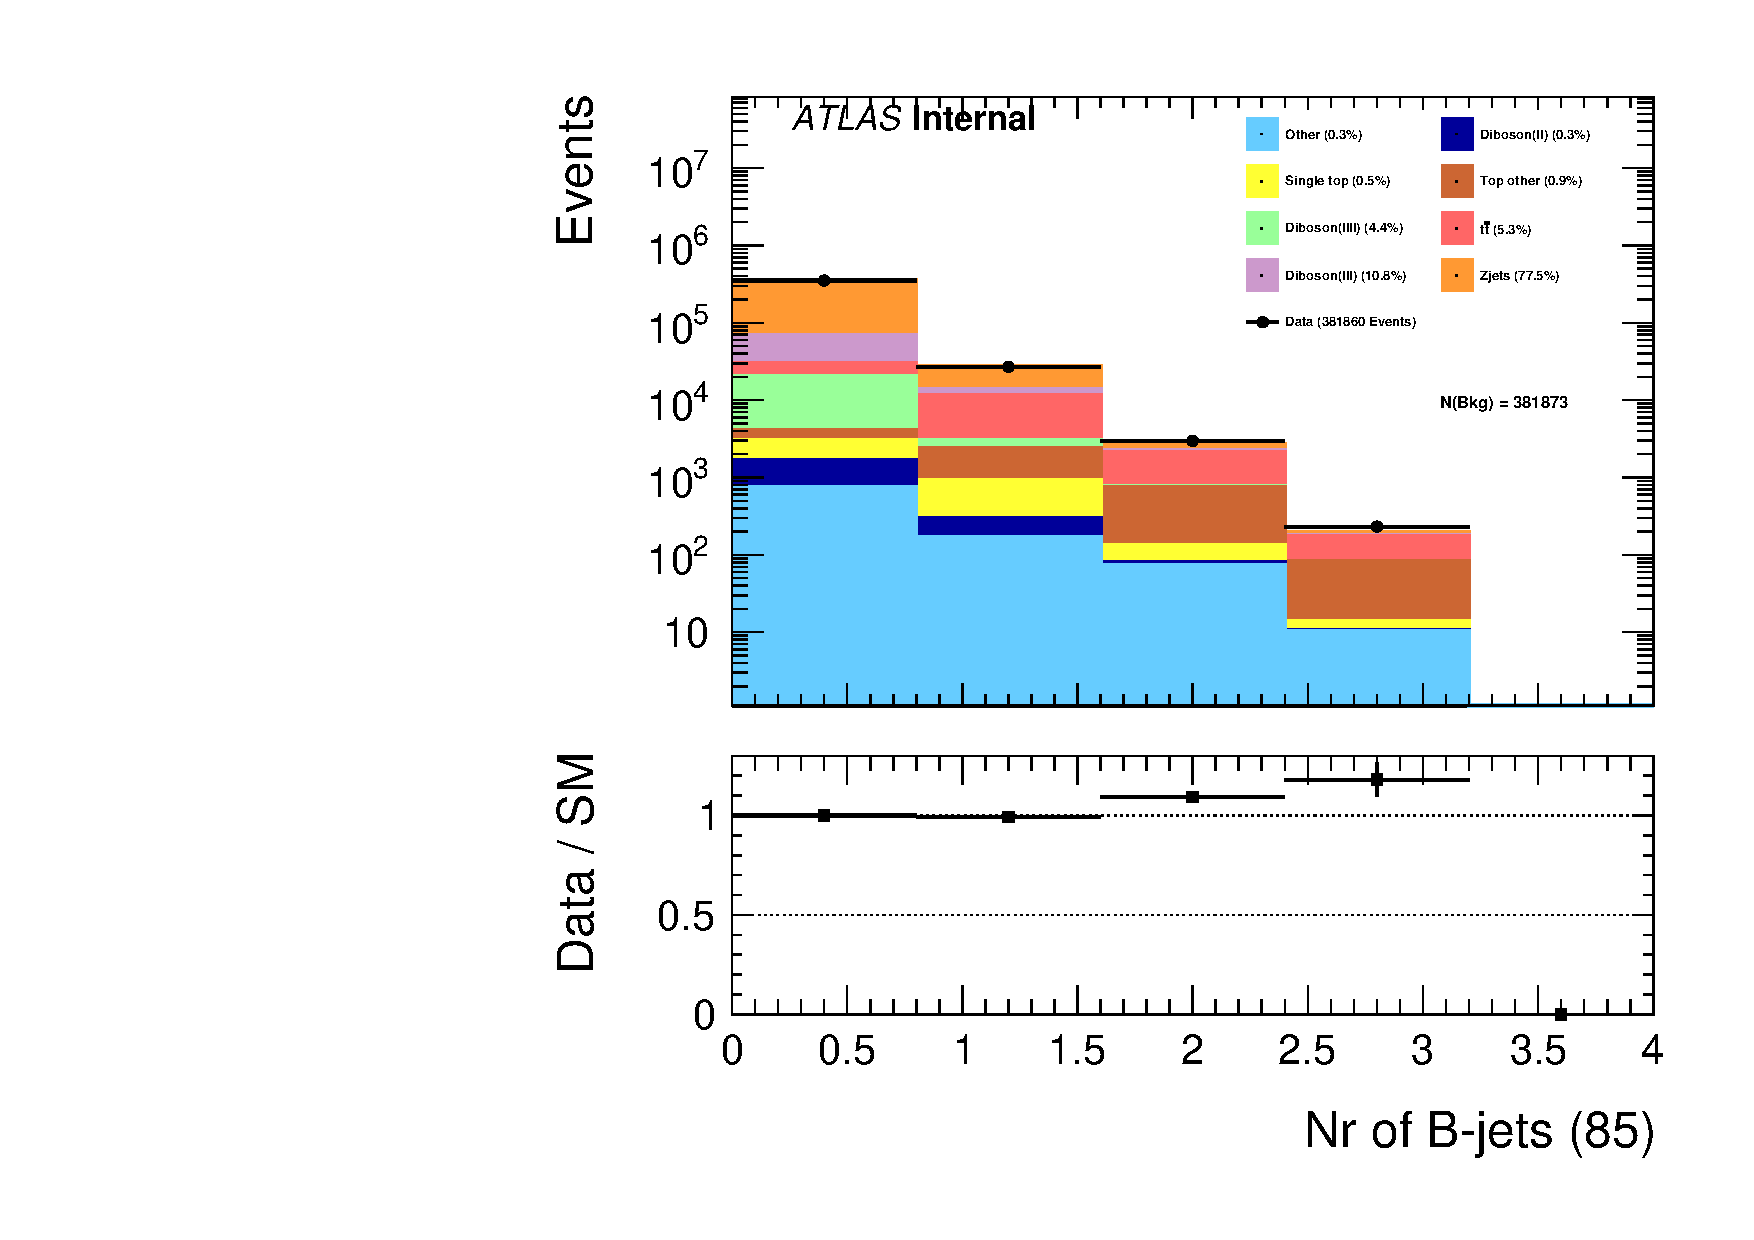
\includegraphics[width=\textwidth]{Figures/FeaturesHistograms/nbjet85.pdf}
        \caption{}
        \label{fig:nbjet85}
    \end{subfigure}
    }
    \caption[\ac{MC} simulated and measured data comparison and event distribution for each channel over the sum of $P_t$
    for the SS pair and the sum over all three leptons added with $E_t^{miss}$. The distribution of number of 
    signal jets and the mass of the leading di-jet pair. Finally, the number of B-jets with $77\%$ and $85\%$ 
    certainty.]{\ac{MC} simulated and measured data comparison and event distribution for each channel over the sum of $P_t$
    for the SS pair \ref{fig:Ht_SS} and the sum over all three leptons added with $E_t^{miss}$
    \ref{fig:Ht_met_Et}. The distribution of number of signal jets \ref{fig:njet_SG} and the mass 
    of the leading di-jet pair \ref{fig:M_jj}. Finally, the number of B-jets with $77\%$ \ref{fig:nbjet77} and $85\%$ 
    \ref{fig:nbjet85} certainty.}
\end{figure}
\newpage
% \begin{figure}[H]
%     \makebox[0.95\linewidth][c]{%
%     \centering
%     \begin{subfigure}{.405\textwidth}
%         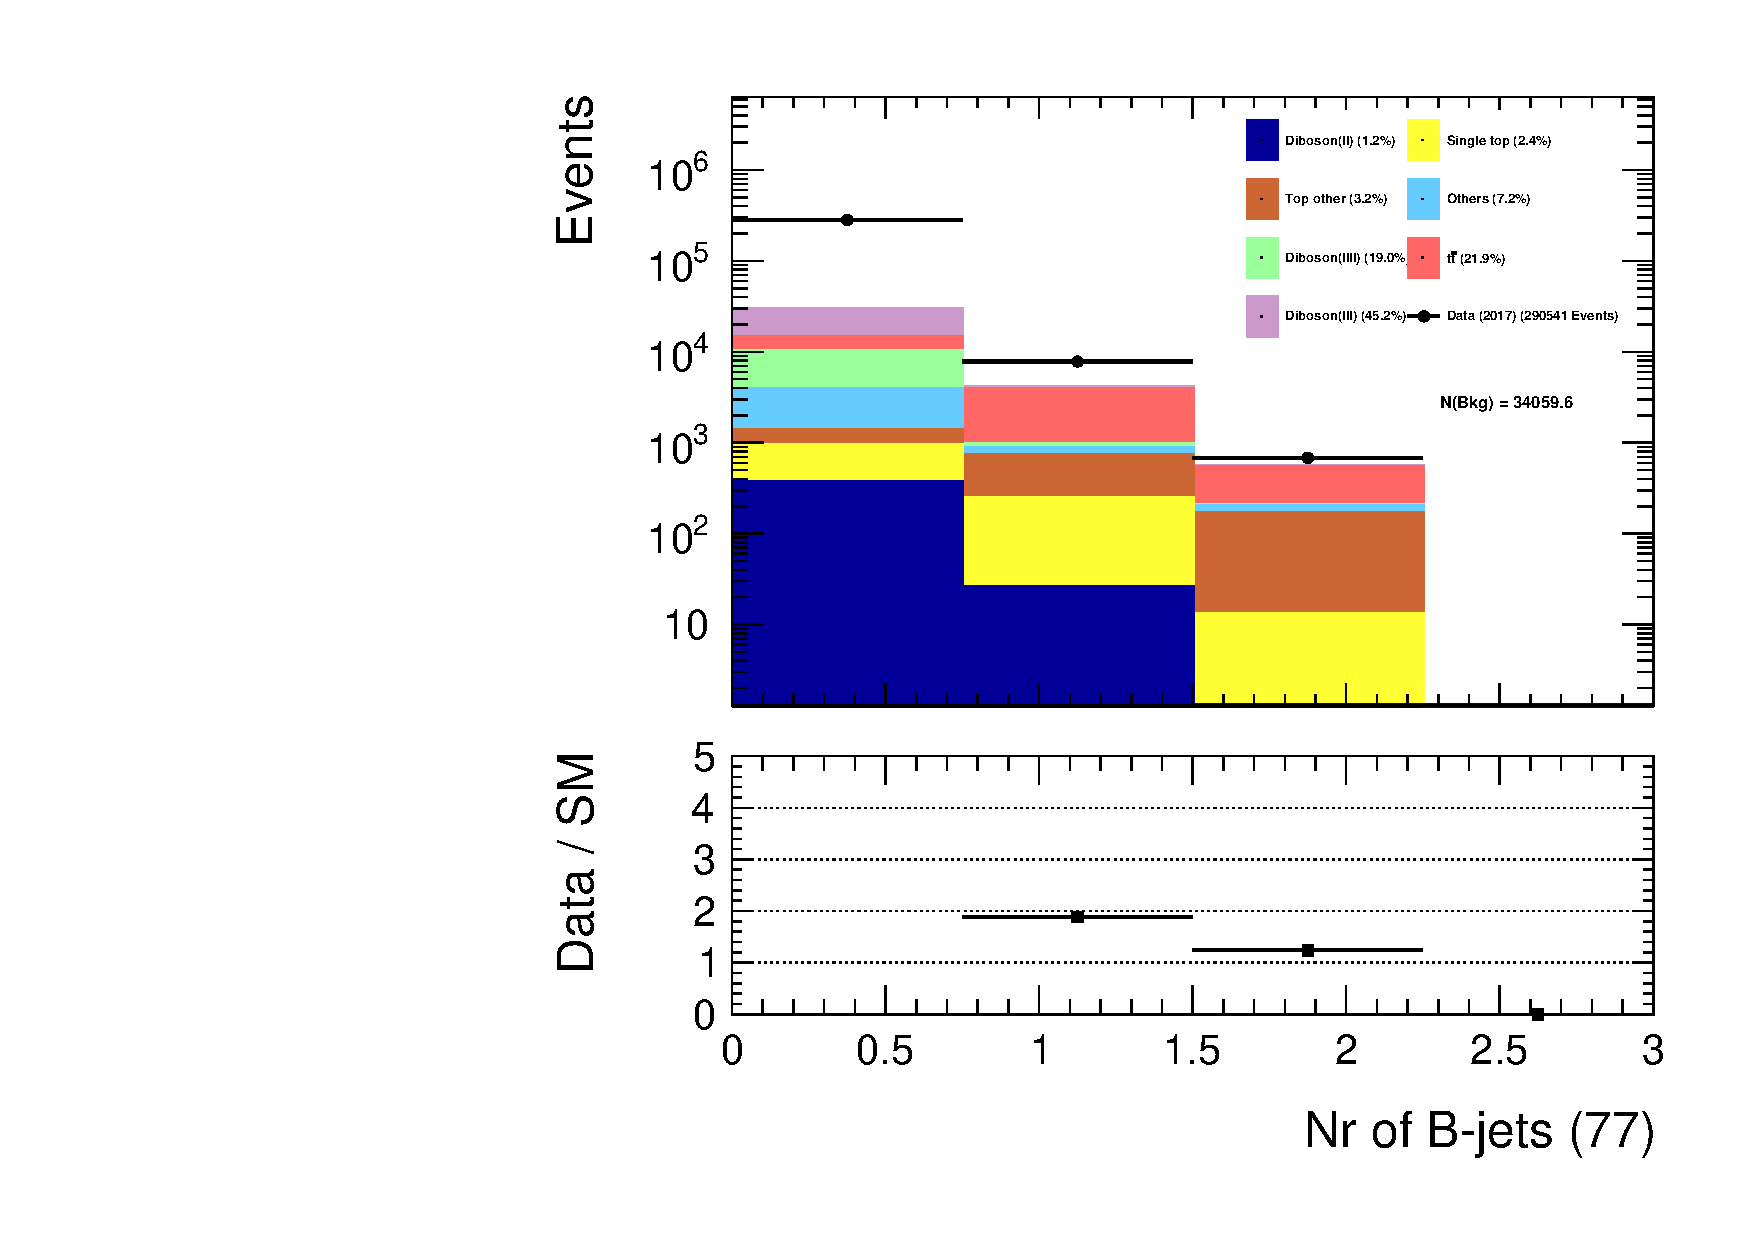
\includegraphics[width=\textwidth]{Figures/FeaturesHistograms/nbjet77.pdf}
%         \caption{}
%         \label{fig:nbjet77}
%     \end{subfigure}
%     \hfill
%     \begin{subfigure}{.525\textwidth}
%         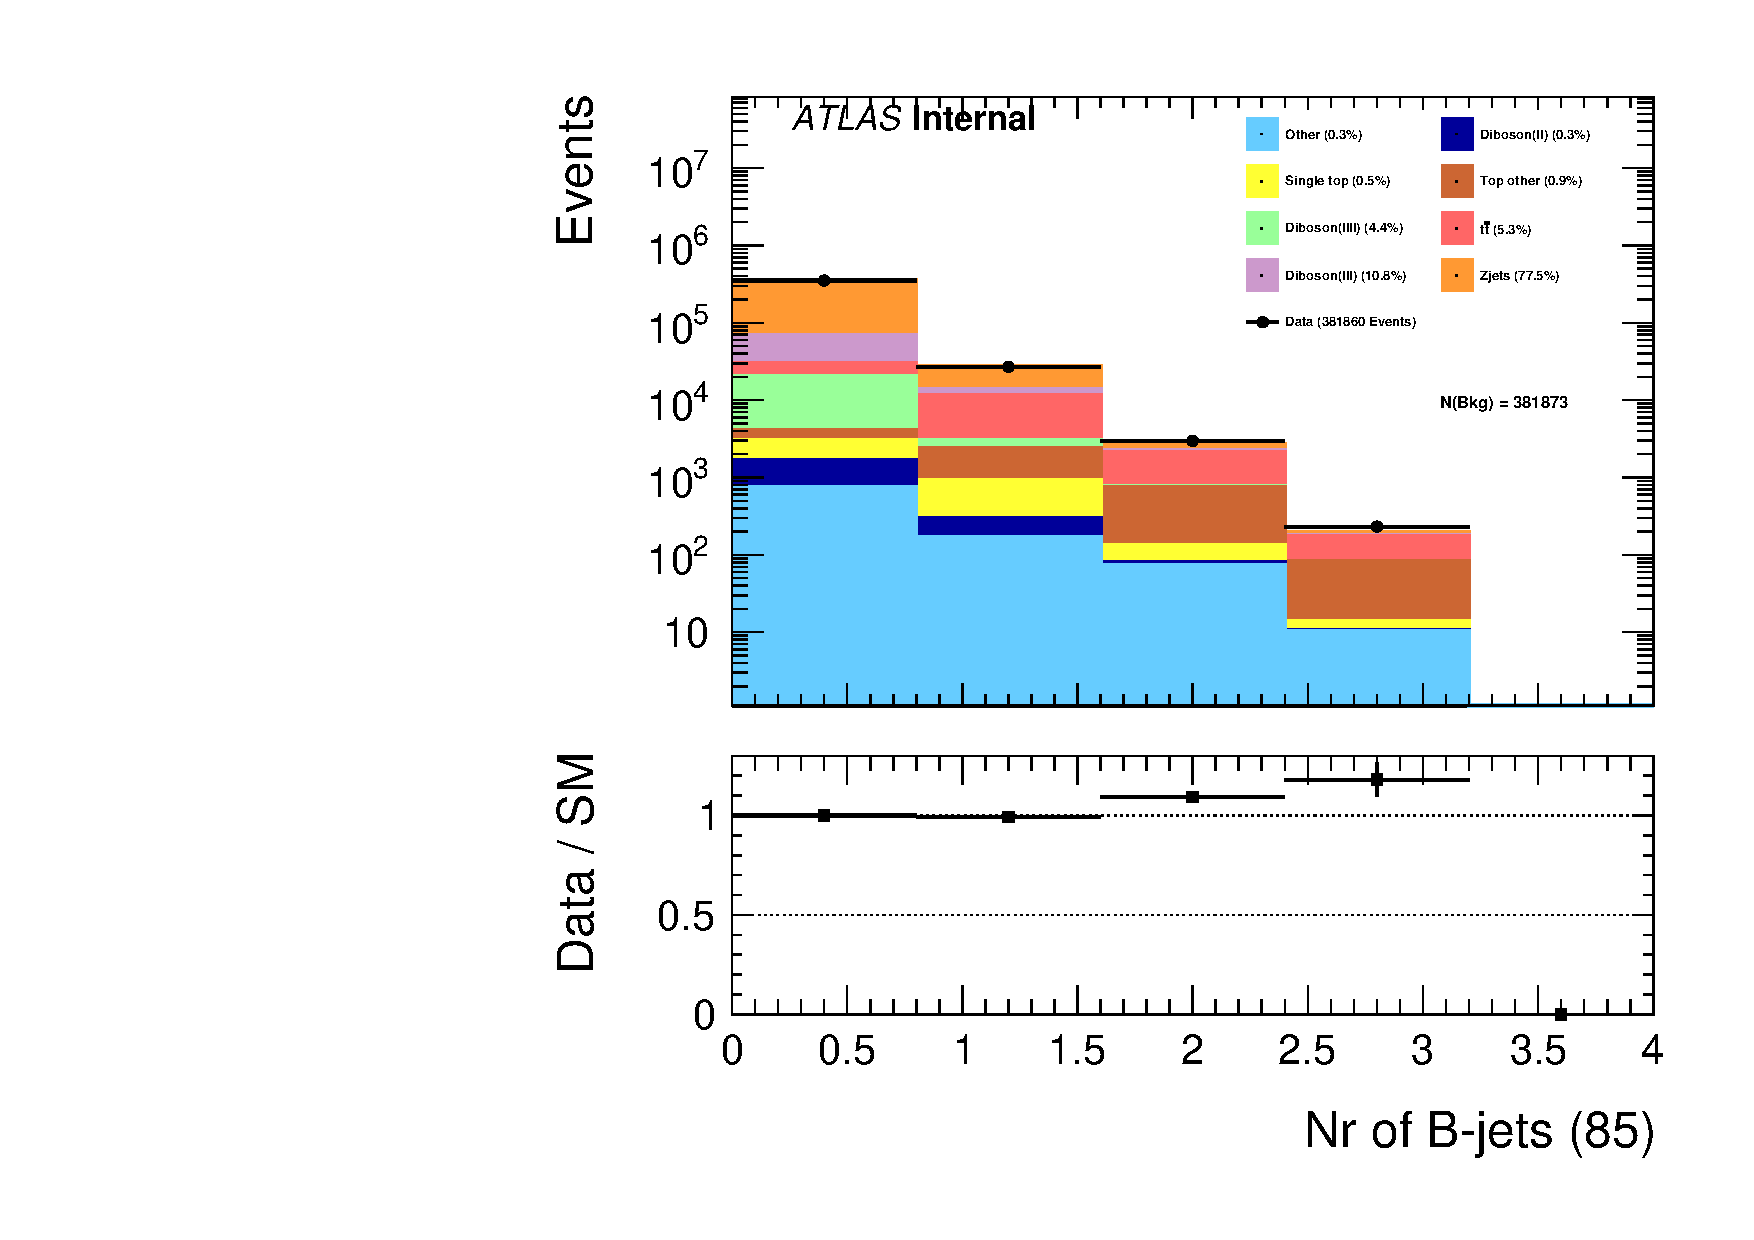
\includegraphics[width=\textwidth]{Figures/FeaturesHistograms/nbjet85.pdf}
%         \caption{}
%         \label{fig:nbjet85}
%     \end{subfigure}
%     }
%     \caption{\ac{MC} and real data comparison and event distribution for each channel over the number of b-jets 
%     with $77\%$ \ref{fig:nbjet77} and $85\%$ \ref{fig:nbjet85} efficiency.}
%     \label{fig:DistLast}
% \end{figure}
\newpage
\subsection{The Selection of Feature}\label{subsec:FeatSelec}

\begin{table}[H]
    \centering
    $
    \begin{array}{cc}
        \hline \text {\textbf{Feature Name} }  & \text {\textbf{Description}} \\
        \hline \hline \text {$P_t$}  & \text {Transverse momentum} \\
        \text {$\eta_t$}  & \text {Pseudo rapidity} \\
        \text {$\phi_t$}  & \text {Azimuthal angle} \\
        \text {$M_T$}  & \text {Transverse mass} \\
        \text {$Charge$}  & \text {\ac{EM} charge} \\
        \text {$Flavour$}  & \text {Particle type} \\
        \text {$E_T^{miss}$}  & \text {Transverse missing energy} \\
        \text{$\phi(miss)$} & \text {Azimuthal angle of the missing energy} \\
        \text{$M_{lll}$} &  \text {Trilepton mass}\\
        \text{$M_{ll}(OSSF)$} & \text {Mass of the \ac{OSSF} pair} \\
        \text{Sig $E_T^{miss}$} & \text {Significance of $E_T^{miss}$} \\
        \text{$H_t(lll)$} &  \text {Sum of $P_t$ for all three leptons }\\
        \text{$H_t(SS)$} &  \text {Sum of $P_t$ for the \ac{SS} pair}\\
        \text{$H_t(lll)+E_T^{miss}$} & \text {-} \\
        \text{$\Delta R$} &  \text {Distance defined in the $\eta-\phi$ space}\\
        \text{Flavor combo} &  \text {Combination of flavors for all three leptons}\\
        \text{Nr of signal Jets} &  \text {Nr of jets passing the signal criteria} \\
        \text{$M_{jj}$} & \text {Mass of the leading jet pair} \\
        \text{Nr of B-jets(77)} & \text {-} \\
        \text{Nr of B-jets(85)} & \text {-} \\
        \hline
    \end{array}
    $
    \caption{A summary and description of all features used in this analysis.}
    \label{table:Features}
\end{table}
\newpage